\documentclass[a4paper,12pt]{article}

%\documentclass[draft, 12pt]{article}
% ================================================== DATOS ==================================================

% Información de la materia
\newcommand{\codMateria}{TA138}
\newcommand{\nombreMateria}{Taller de Diseño de}
\newcommand{\cuatrimestre}{1.\textsuperscript{er} Cuatrimestre}

% Información del TP
\newcommand{\TpTitulo}{Proyecto Integrador -- Checkpoint 4}
\newcommand{\fecha}{\today}
\newcommand{\group}{Grupo 5}

% Información de alumnos
\newcommand{\nombreA}{Lautaro García Vitale}
\newcommand{\padronA}{110028}
\newcommand{\emailA}{lagarciav@fi.uba.ar}

\newcommand{\nombreB}{Santiago Manuel Cabrera}
\newcommand{\padronB}{110445}
\newcommand{\emailB}{smcabrera@fi.uba.ar}

\newcommand{\nombreC}{Francisco Javier Moya}
\newcommand{\padronC}{109899}
\newcommand{\emailC}{fjmoya@fi.uba.ar}

% ================================================== PAQUETES =================================================

% Codificación y lenguaje
\usepackage[utf8]{inputenc}
\usepackage[ddmmyy]{datetime}
\usepackage[language=spanish]{lipsum}
\usepackage[spanish]{datetime2}
\usepackage[T1]{fontenc}
\usepackage[spanish,es-nodecimaldot]{babel}

% -------- CAMBIAR "CUADRO" POR "TABLA" --------
\addto\captionsspanish{
    \renewcommand{\tablename}{Tabla}
}

\usepackage[a4paper,margin=2.5cm]{geometry}
\usepackage{amsmath,amssymb,amsthm,mathtools}
\usepackage{bm}
\usepackage{setspace}
\usepackage{hyperref}
\usepackage{enumitem}

% Márgenes y página
\usepackage{geometry}
\usepackage{fancyhdr}
\usepackage{emptypage}
\usepackage{parskip}

% Encabezado personalizado
\pagestyle{fancy}
\fancyhf{}
\rhead{\group}
\lhead{\TpTitulo}
\cfoot{\thepage}
\setlength{\headheight}{14.5pt}

% Tipografía matemática
\usepackage{mathtools}
\usepackage{amssymb}
\usepackage{amsfonts}
\usepackage{amsthm}
\usepackage{yhmath}
\usepackage{dsfont}
\usepackage{esdiff}
\usepackage{xfrac}
\usepackage{siunitx}
\sisetup{per-mode=reciprocal, separate-uncertainty=true}

% Gráficos y tablas
\usepackage{graphicx}
\usepackage{float}
\usepackage{booktabs}
\usepackage{caption}
\usepackage{subcaption}
\usepackage{multirow}
\usepackage{adjustbox}

% TikZ y gráficos avanzados
\usepackage{pgfplots}
\pgfplotsset{compat=1.18}
\usepackage{tikz}

% Código fuente y resaltado
\usepackage{minted}
\usepackage{tcolorbox}
\definecolor{codebg}{rgb}{0.95,0.95,0.95}  % Color de fondo del código
\usemintedstyle{friendly}                  % Estilo del resaltado de sintaxis
\setminted{
    linenos=true,                          % Numeración de líneas
    bgcolor=codebg,                        % Color de fondo del código
    fontsize=\footnotesize,                % Tamaño de la fuente
    frame=lines,                           % Estilo del marco
    framesep=2mm,                          % Separación del marco
    baselinestretch=1.2,                   % Espaciado entre líneas
    breaklines=true,                       % Romper líneas largas automáticamente
    encoding=utf8,                         % Codificación del archivo
    tabsize=4,                             % Tamaño de la tabulación
}

% Misceláneo
\usepackage{anyfontsize}
\usepackage{xcolor}
\usepackage{url}
\usepackage{comment}
\usepackage{multicol}
\usepackage[numbers,square]{natbib}

% Estilo de bibliografía
\bibliographystyle{IEEEtran}

% ==============================================================================================================
% ==============================================================================================================

\begin{document}

% ================================================== CARÁTULA ==================================================

\pagenumbering{arabic} % Comienza la numeración

\vspace{-1 cm} % La primera hoja tiene que tener menos espaciado

\begin{center}
  \begin{minipage}{0.8 cm}
    
\includegraphics[width=\linewidth]{img/fiuba.png}
  \end{minipage}
  \begin{minipage}{\widthof{\large{\textsc{Universidad de Buenos Aires}}}}
    \centering
    \large{\textsc{Universidad de Buenos Aires}}\\
    \large{\textsc{Facultad de Ingeniería}}\\
    \small{Año 2026 -- \cuatrimestre}
  \end{minipage}
\end{center}
\vspace{10mm}
\begin{center}
  \huge{\underline{\textsc{\nombreMateria}}} \\
  \huge{\underline{\textsc{Circuitos Electrónicos}}} \\
  \vspace{7 pt}
  \Large{\TpTitulo \\}
  \vspace{3mm}
  \large{\group}
\end{center}

\newcommand{\anchopadron}{\widthof{000 000}}
\begin{center}
  \begin{tabular}{l l l}
    \nombreA & \parbox{\anchopadron}{\raggedleft \padronA} & \emailA \\
    \nombreB & \parbox{\anchopadron}{\raggedleft \padronB} & \emailB \\
    \nombreC & \parbox{\anchopadron}{\raggedleft \padronC} & \emailC 
  \end{tabular}
\end{center}
\vspace{8mm}

\begin{center}
\renewcommand{\arraystretch}{1.3}
\begin{tabular}{@{}r p{0.62\textwidth}@{}}
\textbf{Tutor:} & Federico Gabriel D'Angiolo. \\ 
\textbf{Docentes:} & Julio Guillermo Zola, Marcelo Adrián Bruno, Sergio Quinteros y Juan Guido Salaya.
\end{tabular}
\end{center}

\vspace{2em}
\thispagestyle{empty}

\begin{abstract}
En este informe se presenta el análisis, diseño e implementación de un generador de pulsos PWM analógico y el diseño preliminar de una fuente conmutada \textit{buck} a lazo abierto. Para el generador PWM se estudió el funcionamiento de las etapas que determinan la señal triangular y la comparación con una referencia continua, obteniéndose experimentalmente una frecuencia de oscilación de aproximadamente $\SI{118}{\kilo\hertz}$. Para el convertidor \textit{buck}, se desarrolló el modelo ideal en régimen permanente y conducción continua, se determinó la relación entre ciclo de trabajo y tensión de salida, y se dimensionaron los componentes principales para obtener una tensión intermedia cercana a $\SI{9.5}{\volt}$ a partir de una entrada variable entre $\SI{12}{\volt}$ y $\SI{30}{\volt}$. Finalmente, se analizaron las solicitaciones sobre los dispositivos de potencia, los capacitores y el inductor, incluyendo un diseño preliminar del componente magnético mediante el método de Erickson.
\end{abstract}

\newpage


\tableofcontents

\newpage

\section{Introducción}

En el presente informe se detallará el análisis, diseño e implementación de un generador de pulsos PWM analógico. Asimismo, se desarrollará el anñaisis y diseño validado por simulación de una fuente \textit{buck} a lazo abierto.

\section{Diseño del circuito PWM}

Se propone diseñar un generador de pulsos PWM a partir de la siguiente topología. 

\begin{figure}[H]
    \centering
    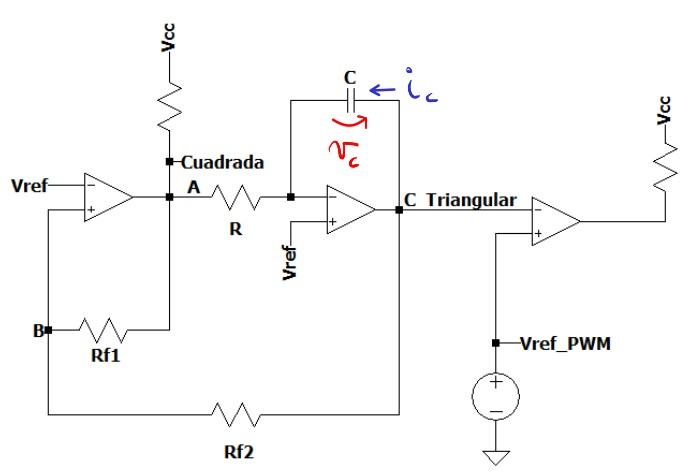
\includegraphics[width=0.8\textwidth]{img/PWM/PWM_topología.jpg}
    \caption{Topología del circuito PWM}
    \label{fig:PWM topologia}
\end{figure}

El circuito consiste en 3 etapas. La etapa 1 es un circuito \textit{Schmitt-trigger} no inversor, el cual generará una señal cuadrada. La segunda etapa es un integrador implementado en un \texttt{OpAmp}, el cual integrará la señal cuadrada para generar una triangular. La última etapa compara la señal triangular con una tensión de referencia variable a través de un potenciómetro. El valor de esta tensión variable permite ajustar el ciclo de trabajo $D$ de los pulsos PWM.

\subsection{Análisis del circuito} 

Es necesario entender cómo varía la frecuencia de las oscilaciones con los componentes para diseñar el circuito. En esta sección, se utilizarán letras minúsculas para las señales variables en el tiempo y letras mayúsculas para las tensiones constantes.

En primer lugar, se buscará la relación entre las señales de los nodos C y A. Al aplicar ley de Ohm a la resistencia $R$ se tiene que $i_c = (V_{ref} -  v_A)/R$, con lo cual

\begin{equation}
    v_c' = i_c/C = -\frac{v_A - V_{ref}}{RC}
\end{equation}

y teniendo en cuenta que $v_{tri} = v_{ref} + v_c$, se llega a 

\begin{equation}
    v_{tri} = -\frac{1}{RC}\int (v_A - V_{ref}) dt + V_{ref}.
    \label{eq:triangular}
\end{equation}

De la \autoref{eq:triangular} se tiene que, si $v_A$ es una señal cuadrada, $v_{tri}$ será una señal triangular montada sobre una tensión continua $V_{ref}$. 

Esta ecuación también indica cómo varían las tensiones del circuito. Si la salida del \textit{Schmitt-trigger} es cero ($v_A = \SI{0}{\volt}$), la tensión $v_{tri}$ crece como una rampa ya que se integra una constante. Eventualmente $v_{tri}$ llegará a un valor lo suficientemente alto para disparar el \textit{Schmitt-trigger}, con lo cual $v_A$ pasará a valer $V_{CC}$. Entonces, la corriente $i_c$ invierte su sentido, el capacitor se descarga y el integrando de la \label{eq:triangular} pasa a ser una constante positiva, por lo que $v_{tri}$ decrece linealmente. Esta tensión decrecerá hasta  llegar al umbral inferior del \textit{Schmitt-trigger}, momento en el cual la tensión $v_A$ volverá a ser cero y el ciclo se repetirá. Este es el principio básico por el cual funciona este circuito.

Para determinar la frecuencia de las oscilaciones es necesario conocer con qué pendiente asciende y desciende la señal triangular, para lo cual se deriva la \autoref{eq:triangular} y se la evalúa en cada semiciclo.

\begin{minipage}{0.45\textwidth}
    \centering
    \begin{equation}
        v_{tri}' = \frac{V_{ref}}{RC} \text{(Subiendo)}
        \label{eq:derivada subiendo}
    \end{equation}
\end{minipage}
\hfill
\begin{minipage}{0.45\textwidth}
    \centering
    \begin{equation}
        v_{tri}' = -\frac{V_
        {CC} - v_{ref}}{RC} \text{(Bajando)}
        \label{eq:derivada bajando}
    \end{equation}
\end{minipage}

Ya que se quiere una señal triangular, las pendientes de subida y bajada deben ser opuestas y de igual módulo. Aplicando estos requerimientos a estas dos ecuaciones se tiene que $V_{ref} = V_{CC}/2$. De esta forma, las pendientes de subida y bajada serán $v_{tri}' = \pm \frac{V_
{CC}}{2RC}$. 

Para determinar la frecuencia de las oscilaciones también es necesario hallar el valor máximo y el valor mínimo de la señal triangular, que se denominarán $V^+$ y $V^-$, respectivamente. De esta forma, cuando $v_A = 0$ la tensión $v_{tri}$ aumenta hasta que $v_{tri} = V^+$, momento en el cual la tensión $V_B$ es igual a $V_{ref}$ y el \textit{Schmitt-trigger} se dispara. Entonces, $v_A$ pasa a valer $V_{CC}$, y la tensión $v_{tri}$ disminuye desde $V^+$ hasta llegar a $V^-$, momento en el cual la tensión $V_B$ es igual a $V_{ref}$ y el \textit{Schmitt-trigger} se vuelve a disparar. 

Para determinar $V^+$ y $V^-$ se busca la tensión del nodo B a partir del divisor resistivo que se forma en las resistencias $R_{f1}$ y $R_{f2}$. Se tiene entonces que

\begin{equation}
    V_B = \frac{R_{f1}}{R_{f1} + R_{f2}} \cdot (v_{tri} - v_A) + v_A.
    \label{eq:nodo B}
\end{equation}

A partir de esta ecuación, se evalúan los dos casos mencionados previamente: cuando $v_A = 0$, $v_{tri} = V^+$ y $V_B = V_{ref}$ y cuando $v_A = V_{CC}$, $v_{tri} = V^-$ y $V_B = V_{ref}$. 

\begin{minipage}{0.45\textwidth}
    \centering
    \begin{equation*}
        V_{ref} = \frac{R_{f1}}{R_{f1} + R_{f2}} \cdot V^+
    \end{equation*}
\end{minipage}
\hfill
\begin{minipage}{0.45\textwidth}
    \centering
    \begin{equation*}
        V_{ref} = \frac{R_{f1}}{R_{f1} + R_{f2}} \cdot (V^- - V_{CC}) + V_{CC}
    \end{equation*}
\end{minipage}

Se despejan entonces $V^+$ y $V^-$ de cada ecuación, teniendo en cuenta que $V_{CC} = 2V_{ref}$ como se estableció previamente.

\begin{minipage}{0.45\textwidth}
    \centering
    \begin{equation}
        V^+ = (1 + \frac{R_{f2}}{R_{f1}}) \cdot V_{ref}
        \label{eq:V+}
    \end{equation}
\end{minipage}
\hfill
\begin{minipage}{0.45\textwidth}
    \centering
    \begin{equation}
        V^- = (1 - \frac{R_{f2}}{R_{f1}}) \cdot V_{ref}
        \label{eq:V-}
    \end{equation}
\end{minipage}


\begin{equation}
    \Delta V = V^+ - V^- = 2 \frac{R_{f2}}{R_{f1}} V_{ref}
    \label{eq:delta V}
\end{equation}
De esta forma, la triangular debe recorrer las tensiones $V^-$ a $V^+$ en la mitad del período, es decir, debe aumentar $\Delta V = V^+ - V^-$ en $T/2$. De las ecuaciones \ref{eq:V+} y \ref{eq:V-} puede obtenerse que $\Delta V = 2 \frac{R_{f2}}{R_{f1}} V_{ref}$. Puede relacionarse el rango de tensiones a recorrer con el tiempo que lleva recorrerlas a través de la derivada (ecuaciones \ref{eq:derivada subiendo} y \ref{eq:derivada bajando}). Se tiene entonces que

\begin{equation*}
    \frac{T}{2} = \frac{\Delta V}{v_{tri}'} = \frac{2 R_{f2}/R_{f1} V_{ref}}{V_{ref}/RC} = 2 RC \frac{R_{f2}}{R_{f1}}. 
\end{equation*}


Se despeja entonces $f = 1/T$.

\begin{equation}
    f = \frac{1}{4RC} \cdot \frac{R_{f1}}{R_{f2}}
    \label{eq:frecuencia}
\end{equation}

\subsection{Diseño y elección de componentes}

En primer lugar, ya que el circuito será alimentado desde una batería cuya tensión podría variar entre $\SI{12}{\volt}$ y $\SI{30}{\volt}$, se eligió un regulador LM7809 para mantener la tensión constante en $\SI{9}{\volt}$ y alimentar al resto del circuito. Esto fija $V_{CC} = \SI{9}{\volt}$ y $V_{ref} = \SI{4,5}{\volt}$. En segundo lugar, se eligió que la amplitud pico a pico de la señal triangular fuera de \SI{1}{\volt}, con lo cual de la \autoref{eq:delta V} se tiene que

\begin{equation*}
    \frac{R_{f2}}{R_{f1}} = \frac{1}{9}.
\end{equation*}

En principio se eligieron $R_{f1} = \SI{510}{\kilo \Omega}$ y $R_{f2} = \SI{56}{\kilo \Omega}$, pero finalmente se usaron $R_{f1} = \SI{560}{\kilo \Omega}$ y $R_{f2} = \SI{56}{\kilo \Omega}$ ya que no fue posible adquirir resistores de los valores originales. 

Luego, se busca una frecuencia de trabajo de aproximadamente \SI{135}{\kilo \hertz}. Se eligió un capacitor de \SI{120}{\pico \farad} y se despejó la resistencia $R$ de la \autoref{eq:frecuencia}, dando un valor de $R = \SI{154,3}{\kilo \Omega}$, cuyo valor comercial más cercano es $\SI{150}{\kilo \Omega}$. Estos valores dan, finalmente, una frecuencia de oscilación de $f = \SI{138,8}{\kilo \hertz}$.

Para el amplificador operacional se utilizó el integrado TL072, el cual presenta un slew rate lo suficientemente grande para esta aplicación. Además, es un circuito específicamente diseñado para minimizar el ruido, lo que lo hace preferible por sobre otros amplificadores de la familia TL0XX. En el encapsulado se incluyen 2 amplificadores, uno de los cuales fue utilizado como integrador. El segundo fue utilizado para generar la tensión $V_{ref} = \SI{4,5}{\volt}$ con un divisor resistivo y un seguidor. 

Para el comparador se eligió el LM393, de amplia disponibilidad y con requisitos suficientes para esta aplicación. Se procuró usar un comparador lo suficientemente rápido para la frecuencia de trabajo y que pudiera alcanzar todo el rango de tensiones. 

Según la hoja de datos del LM393, la corriente máxima que puede ingresar al comparador es $I_{MAX} = \SI{1,5}{\ampere}$. Es necesario, entonces, poner resistencias de \textit{pull-up} para limitar esta corriente. La resistencia de \textit{pull-up} mínima es $R_{PU} = V_{CC}/I_{MAX} = \SI{1,5}{\kilo \Omega}$, pero se optó por resistencias de $\SI{5,1}{\kilo \Omega}$ ya que mejoraban el desempeño del circuito. 

\subsection{Simulación y diseño del PCB}

\begin{figure}[H]
    \centering
    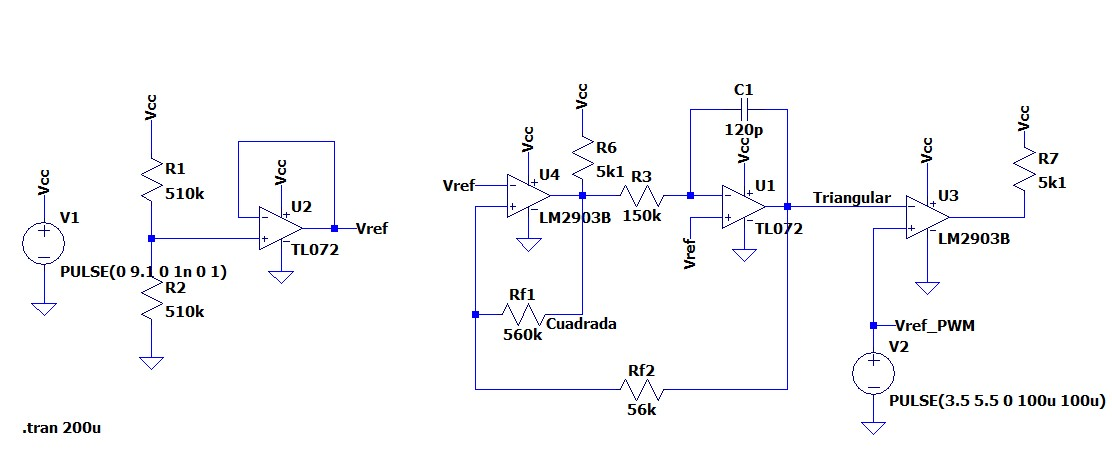
\includegraphics[width=0.8\textwidth]{img/PWM/PWM_simulación.jpg}
    \caption{Simulación en \textit{LTSpice}}
    \label{fig:circuito simulacion}
\end{figure}

Se utilizó el circuito de la \autoref{fig:circuito simulacion} para simular el PWM en \textit{LTSpice}. Los resultados pueden verse en la \autoref{fig:señales}.


\begin{figure}[H]
    \centering
    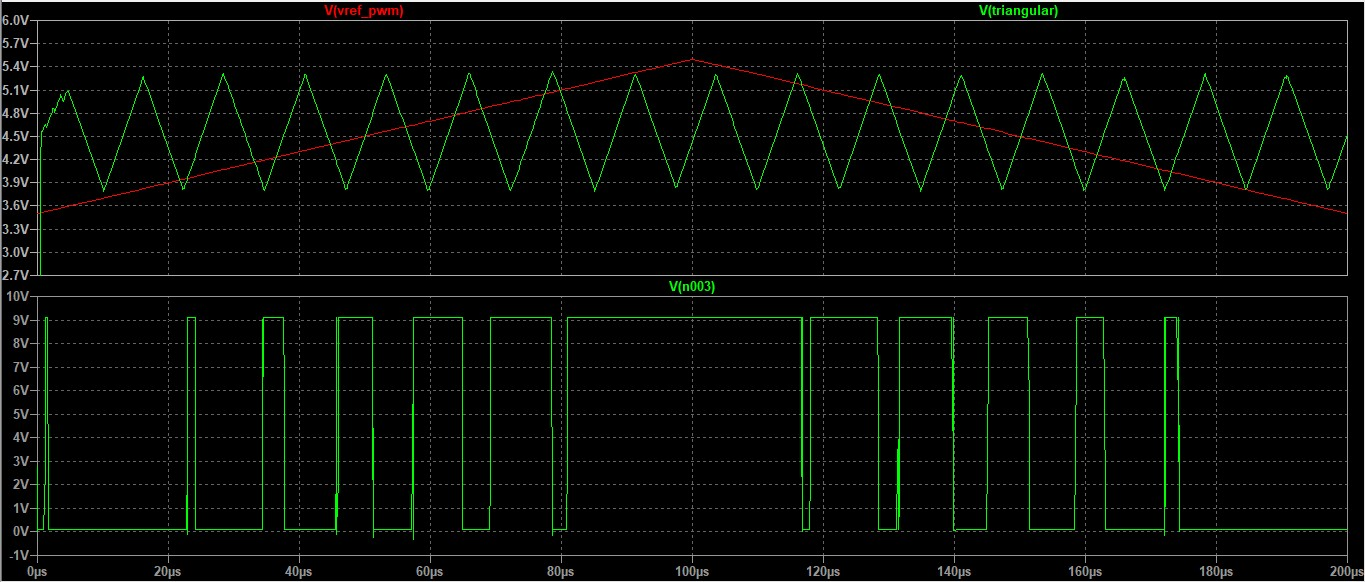
\includegraphics[width=0.95\textwidth]{img/PWM/PWM_señales.jpg}
    \caption{Resultados de la simulación}
    \label{fig:señales}
\end{figure}

Puede apreciarse que el PWM funciona según lo esperado, excepto por la frecuencia de oscilación, la cual es $f = \SI{80}{\kilo \hertz}$. Se decidió entonces reemplazar el capacitor C de $\SI{120}{\pico \farad}$ por uno más chico de $\SI{47}{\pico \farad}$. 

La causa de esta discrepancia es el modelo del comparador y su tiempo de respuesta. El tiempo de respuesta es el tiempo que tardan en propagarse los cambios en la entrada a la salida. Es decir, ante un cambio en las entradas del comparador, el cambio correspondiente en la salida solo se hará efectivo un tiempo de respuesta luego. Según su hoja de datos, el LM393 presenta un tiempo de respuesta de $\SI{1,3}
{\micro s}$, lo que resulta comparable con el período de la señal y explica que las oscilaciones sean más lentas. 

\begin{figure}[H]
    \centering
    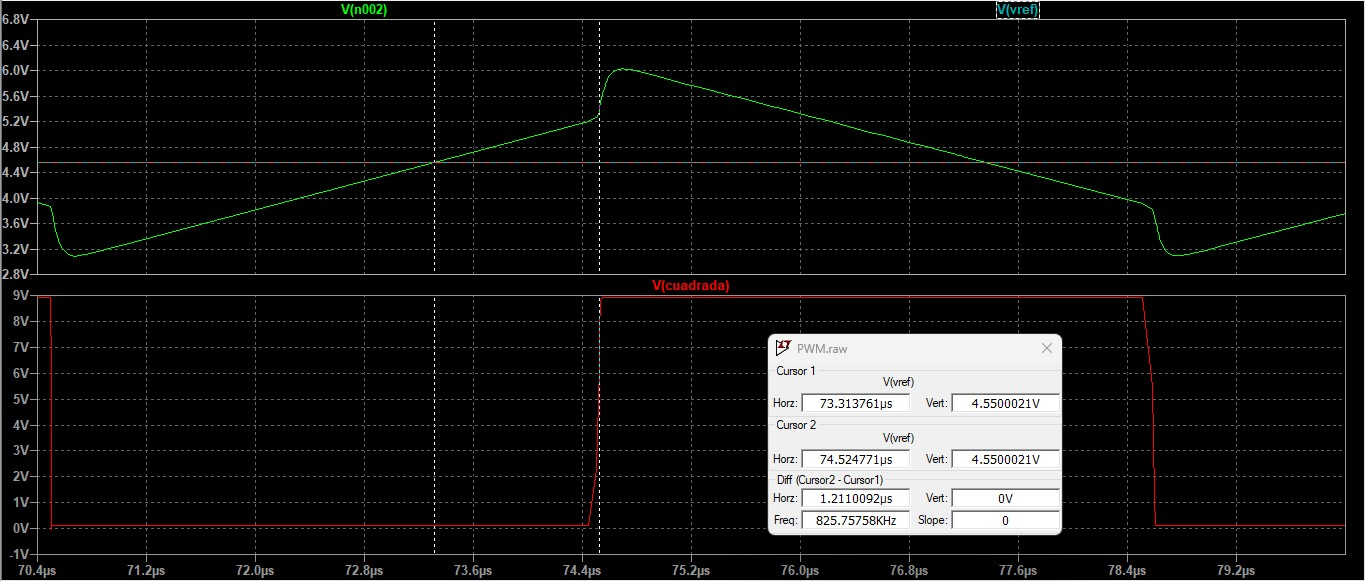
\includegraphics[width=0.95\textwidth]{img/PWM/Tiempo de respuesta.jpg}
    \caption{Tiempo de respuesta del comparador}
    \label{fig:tiempo de respuesta}
\end{figure}

En la \autoref{fig:tiempo de respuesta} puede observarse que el tiempo de respuesta del comparador es de aproximadamente $\SI{1,2}{\micro s}$ en la simulación. Las dos imágenes en el panel superior son las entradas del comparador. Vemos que cuando se cruzan, la salida del comparador no cambia instantáneamente. También se observa en la simulación que la salida del comparador no llega a los valores de la alimentación ($V_{CC}$ y \texttt{GND}). Si bien se acerca bastante, esto es otra fuente de discrepancias ya que no fue considerada en el análisis teórico. Estos dos efectos tienden a hacer al circuito más lento, lo que explica la necesidad de un nuevo capacitor.


Con el circuito ya simulado, se diseñó y construyó el PCB. 

\begin{figure}[H]
    \centering
    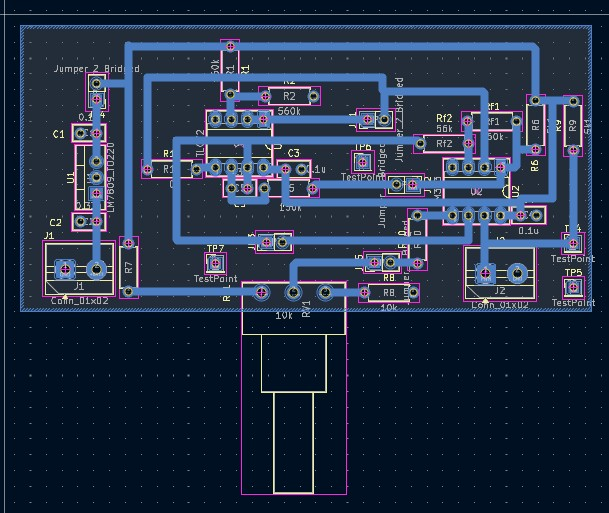
\includegraphics[width=0.8\textwidth]{img/PWM/PWM PCB.jpg}
    \caption{PCB diseñado}
    \label{fig:PCB}
\end{figure}

\begin{figure}[H]
    \centering
    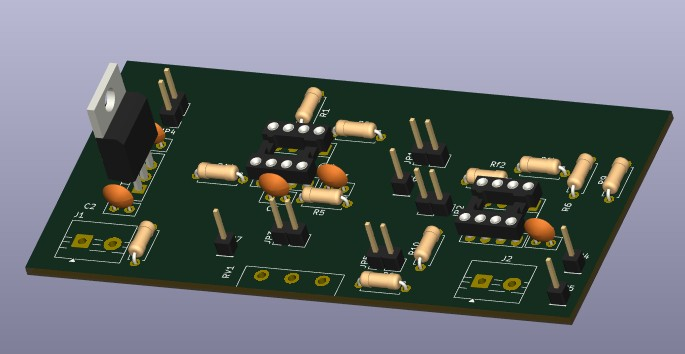
\includegraphics{img/PWM/PWM PCB3D.jpg}
    \caption{PCB diseñado}
    \label{fig:PCB 3D}
\end{figure}

\subsection{Mediciones}

Con el circuito ya armado se midieron las señales del circuito con un osciloscopio. Fue necesario configurar la punta y el equipo en \texttt{X10} para que la punta no filtrara los armónicos de las frecuencias más elevadas. 

En un primer momento se observó que la frecuencia de las oscilaciones era excesivamente alta ($f = \SI{200}{\kilo \hertz}$), por lo que nuevamente se ajustó el valor del capacitor a uno de $\SI{100}{\pico \farad}$, lo que redujo la frecuencia a $f = \SI{118}{\kilo \hertz}$. Hecho este cambio, se hicieron mediciones con el osciloscopio para obtener los siguientes gráficos. 

\begin{minipage}{0.45\textwidth}
    \centering
    \begin{figure}[H]
        \centering
        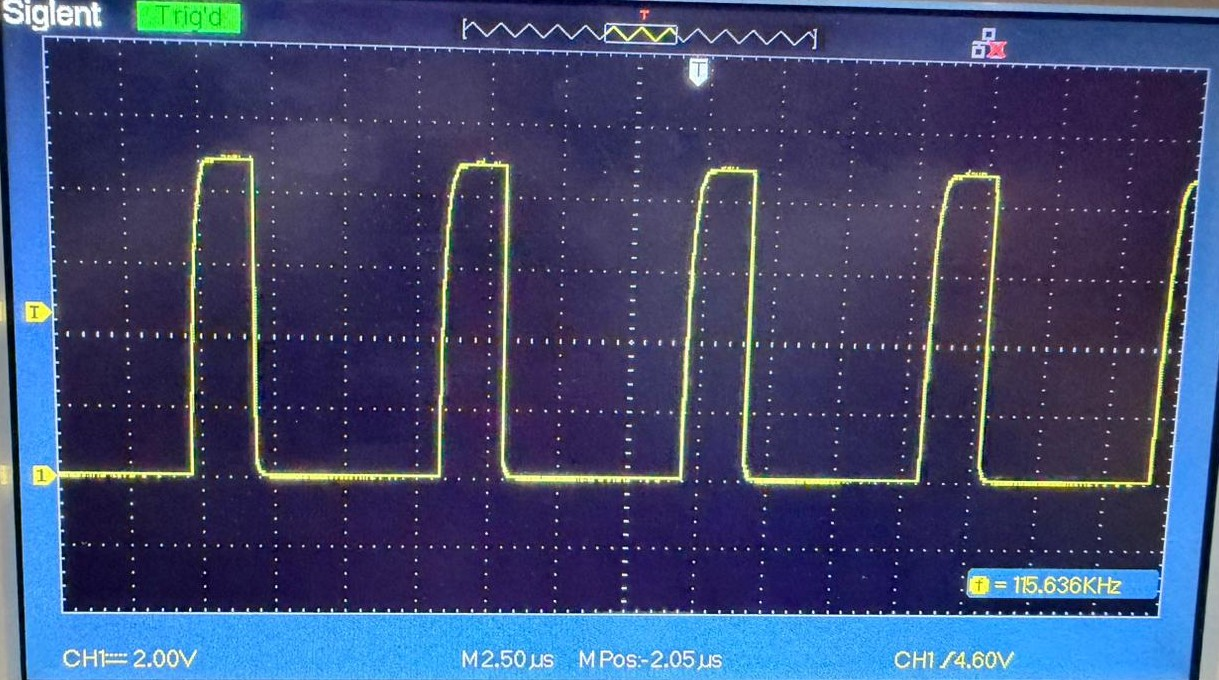
\includegraphics[width=0.9\textwidth]{img/PWM/DC_chico.jpeg}
        \caption{Salida con \textit{duty cycle} menor}
        \label{fig:DC chico}
    \end{figure}
\end{minipage}
\hfill
\begin{minipage}{0.45\textwidth}
    \centering
    \begin{figure}[H]
        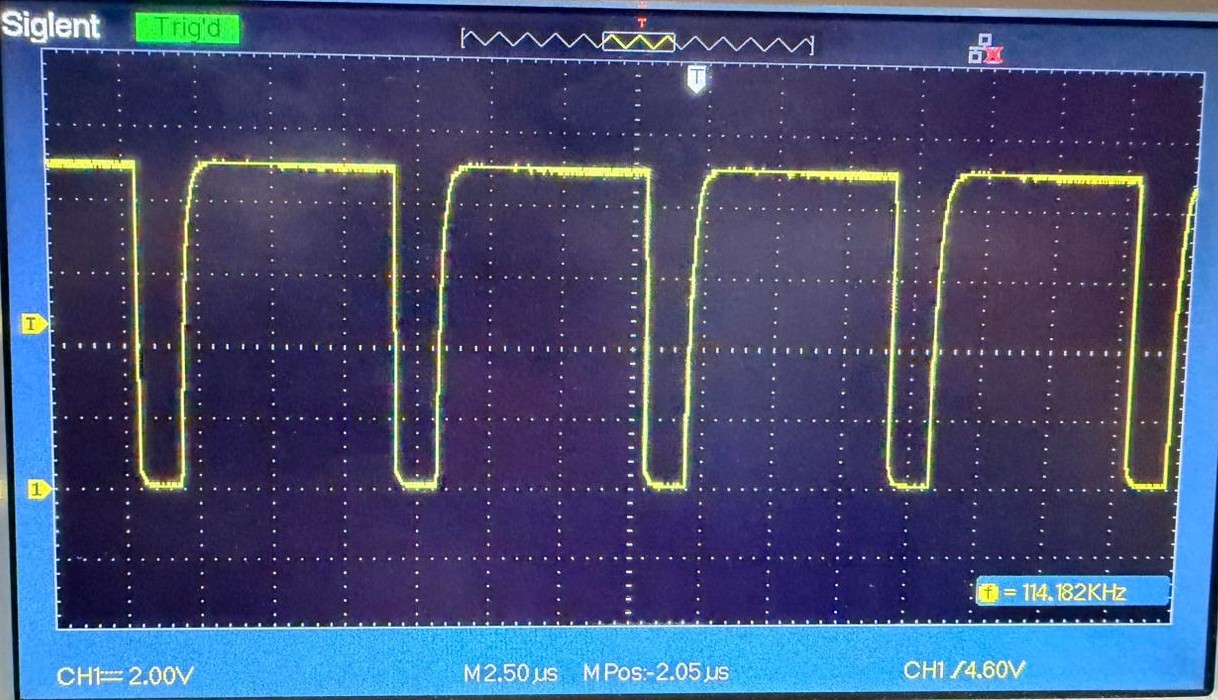
\includegraphics[width=0.9\textwidth]{img/PWM/DC_grande.jpeg}
        \caption{Salida con \textit{duty cycle} mayor}
        \label{fig:DC grande}
    \end{figure}
\end{minipage}

\begin{figure}[H]
    \centering
    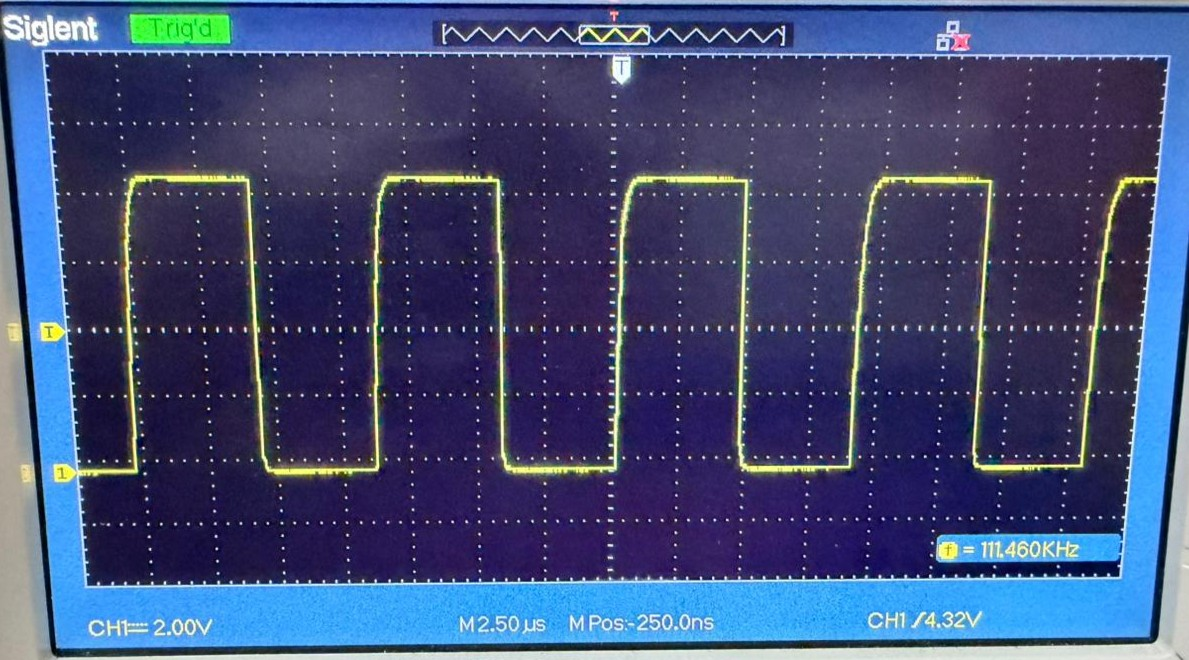
\includegraphics[width=0.9\textwidth]{img/PWM/Cuadrada.jpeg}
    \caption{Señal cuadrada}
    \label{fig:Cuadrada}
\end{figure}

\begin{figure}[H]
    \centering
    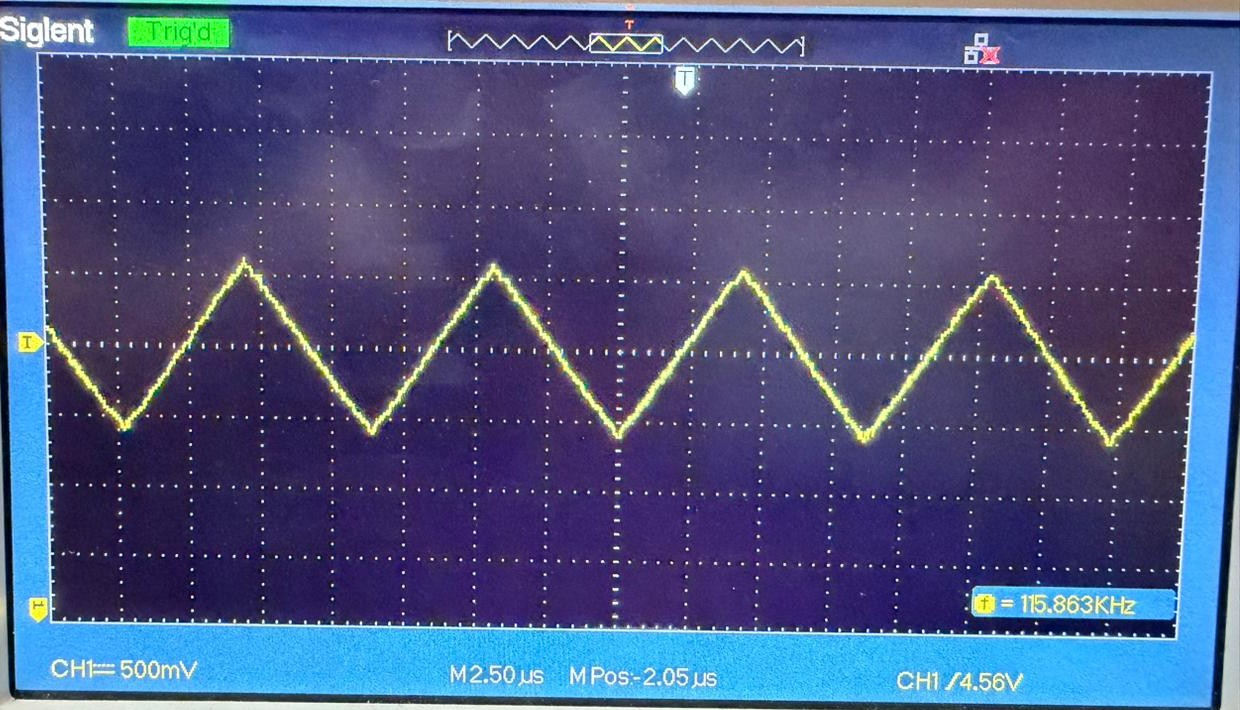
\includegraphics[width=0.9\textwidth]{img/PWM/Triangular.jpeg}
    \caption{Señal triangular}
    \label{fig:triangular}
\end{figure}


\section{Diseño del \textit{Buck Converter}}

El regulador \textit{buck} es una fuente conmutada capaz de generar una tensión media de salida menor que la tensión de entrada, manteniendo una eficiencia considerablemente alta. En este proyecto se utiliza como pre-regulador conmutado, tomando la tensión de batería $V_{IN}$ y generando una tensión intermedia $V_{REG}$ que alimenta al regulador lineal \textit{LDO}.

La especificación del sistema establece que la tensión de entrada puede variar entre

\begin{equation}
    12\ \si{\volt} \leq V_{IN} \leq 30\ \si{\volt}
\end{equation}

mientras que la tensión regulada por el \textit{buck} debe ser aproximadamente

\begin{equation}
    V_{REG} \approx 9.5\ \si{\volt}.
\end{equation}

Por lo tanto, el convertidor debe operar como un reductor de tensión para todo el rango de entrada. El análisis inicial se realiza considerando componentes ideales, operación en régimen permanente (\textit{steady-state}), conducción continua en el inductor (\textit{Continuous Conduction Mode}) y poco \textit{ripple} en la tensión de salida.

\subsection{Circuito ideal del convertidor}

En su forma ideal, el \textit{buck converter} está compuesto por dos interruptores complementarios, un inductor $L$, un capacitor de salida $C$ y una carga equivalente $R$ (ver fig. \ref{fig:buck-converter}). 

\begin{figure}[H]
  \centering
  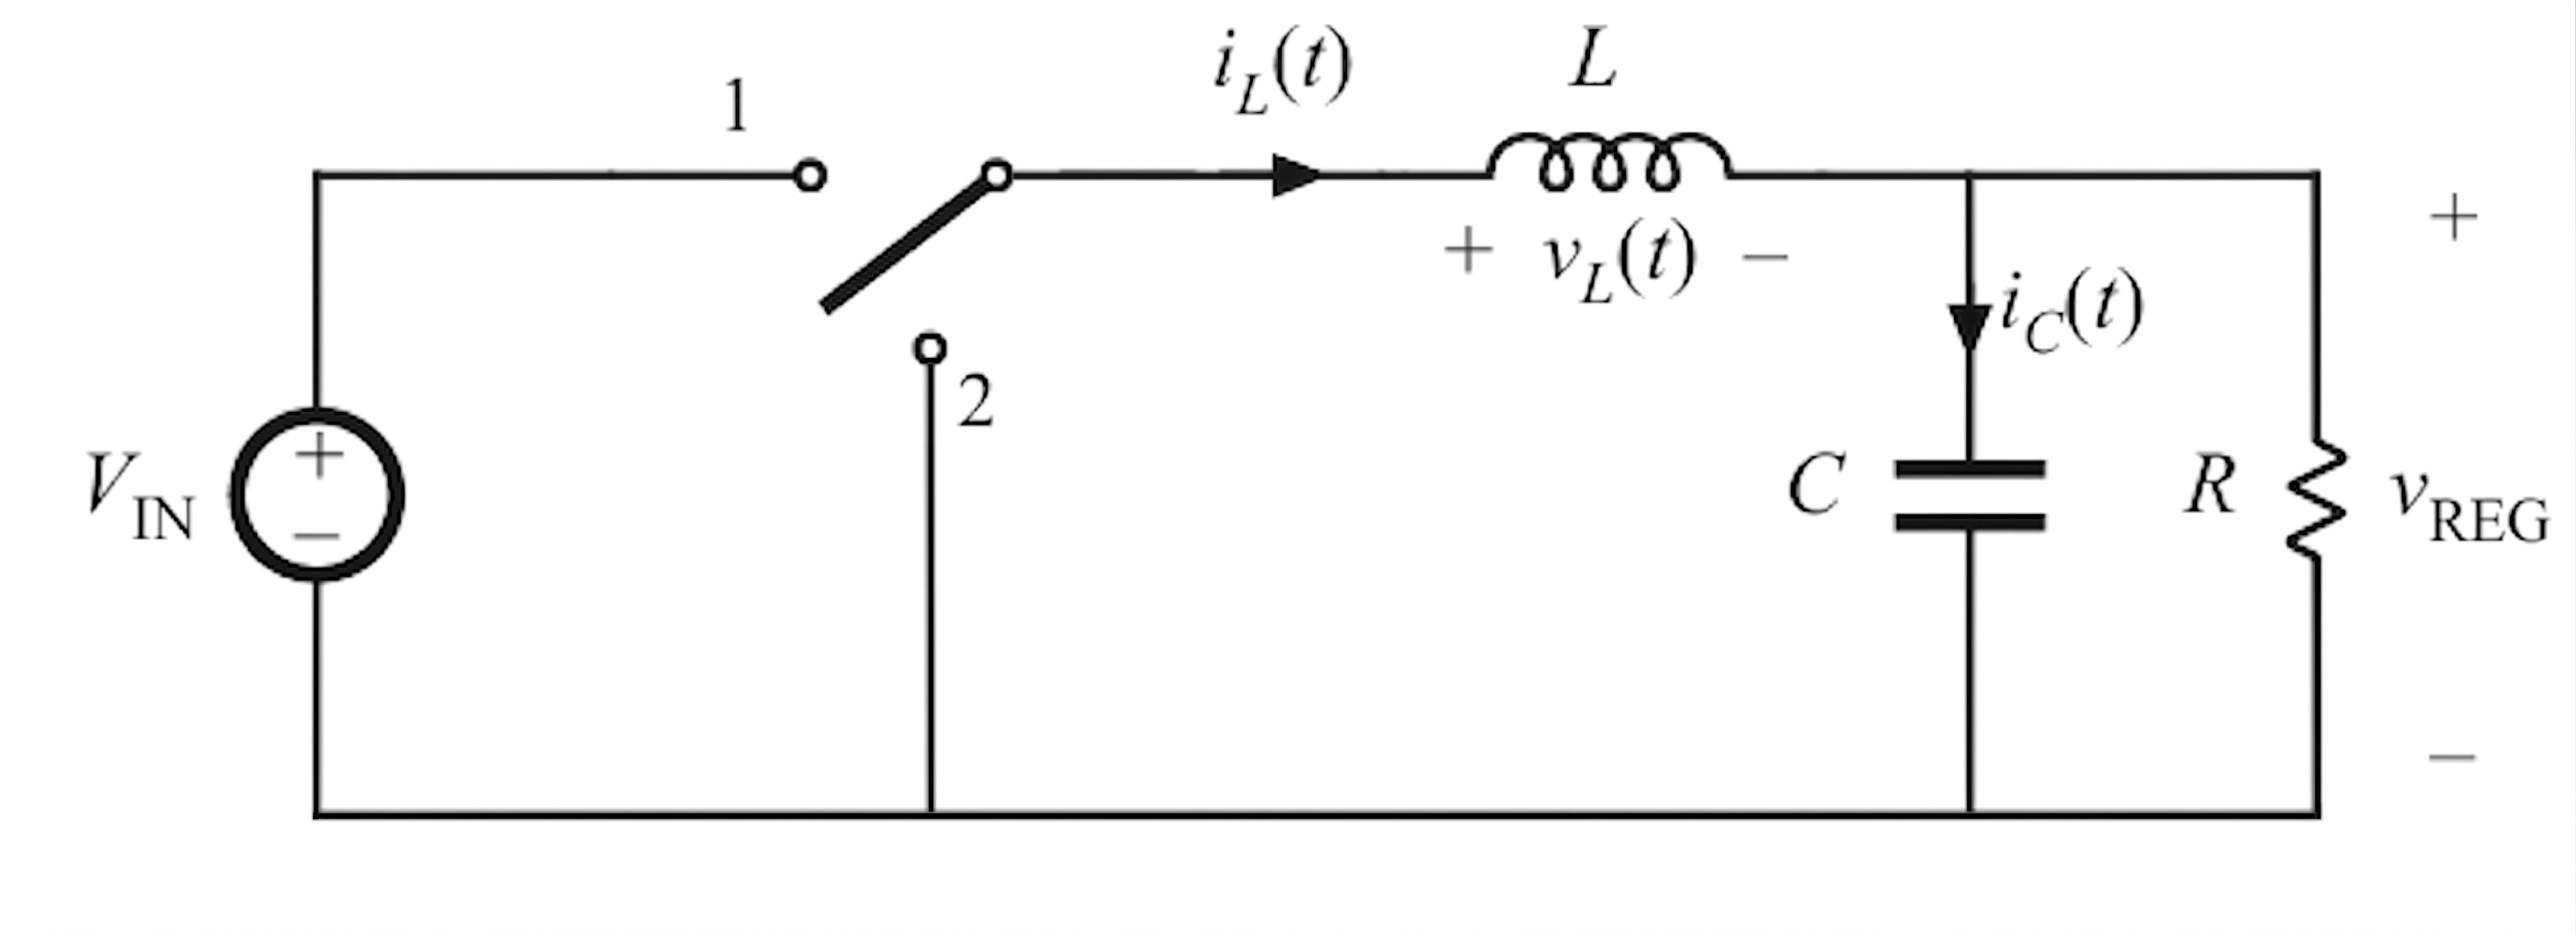
\includegraphics[width=0.65\textwidth]{img/buck-converter.png}
  \caption{Circuito del \textit{buck converter} con las corrientes ($i_L(t)$ e $i_C(t)$) y tensiones ($v_L(t)$ y $v_\text{REG}(t)$) del inductor y capacitor identificadas.}
  \label{fig:buck-converter}
\end{figure}


Los interruptores operan de manera complementaria: cuando el interruptor superior se encuentra cerrado, el interruptor inferior permanece abierto; cuando el superior se abre, el inferior se cierra. De esta forma, el nodo de conmutación alterna periódicamente entre dos niveles de tensión.

El inductor no permite cambios instantáneos de corriente, por lo que transforma la tensión pulsante del nodo de conmutación en una corriente con variaciones suaves. El capacitor, por su parte, no permite cambios instantáneos de tensión, por lo que filtra la componente alterna de la corriente del inductor y mantiene aproximadamente constante la tensión de salida $v_\text{REG}(t)$.

La idea central del regulador es la siguiente: los interruptores generan una señal pulsante, mientras que el filtro $LC$ extrae su valor medio y atenúa las componentes de alta frecuencia. En régimen permanente, si el regulador opera en \textit{continuous conduction mode} (CCM), la corriente del inductor nunca llega a cero dentro del período de conmutación.

\subsection{Hipótesis de análisis}

Para realizar el análisis ideal del regulador se adoptan las siguientes hipótesis:

\begin{itemize}
    \item Los dos interruptores son ideales, por lo que no presentan caída de tensión en conducción ni pérdidas durante la conmutación.
    \item El inductor es ideal, por lo que no presenta resistencia serie ni pérdidas magnéticas.
    \item El capacitor es ideal, por lo que no presenta resistencia serie equivalente (ESR) ni corriente de fuga.
    \item El convertidor opera en régimen permanente, es decir, las formas de onda se repiten ciclo a ciclo.
    \item La corriente del inductor opera en \textit{continuous conduction mode} (CCM), es decir, siempre pasa corriente por el mismo.
    \item Se adopta la aproximación de \textit{small ripple}, por lo que la tensión de salida se considera prácticamente constante durante un período de conmutación.
\end{itemize}

La última hipótesis permite escribir

\begin{equation}
    v_\text{REG}(t) \approx V_\text{REG},
\end{equation}

donde $V_\text{REG}$ es el valor medio de la tensión de salida del \textit{buck}. Esta aproximación no implica que el ripple sea nulo, sino que su amplitud es suficientemente pequeña como para no afectar el análisis de primer orden.

Bajo estas hipótesis, el comportamiento del convertidor puede estudiarse analizando sus dos estados de conmutación dentro de un período $T_s$.

\subsection{Estados de conmutación}

Sea $T_s$ el período de conmutación y $D$ el ciclo de trabajo del PWM. Dentro de cada período, el convertidor alterna entre dos estados o posiciones de conmutación.

Durante una fracción $D T_s$ del período, el nodo de conmutación queda conectado a la tensión de entrada $V_{IN}$. Durante el intervalo restante, de duración $(1-D)T_s$, el nodo de conmutación queda conectado a masa.

Estas dos posiciones determinan la tensión aplicada sobre el inductor y, en consecuencia, la evolución de su corriente.

\subsubsection{Primera posición: carga del inductor}

Durante el intervalo

\begin{equation}
    0 < t < D T_s,
\end{equation}

el nodo de conmutación queda conectado a $V_{IN}$, como se muestra en la fig. \ref{fig:first-position}. Por lo tanto, la tensión aplicada sobre el inductor resulta

\begin{equation}
    v_L(t) = V_{IN} - v_\text{REG}(t).
\end{equation}


\begin{figure}[H]
  \centering
  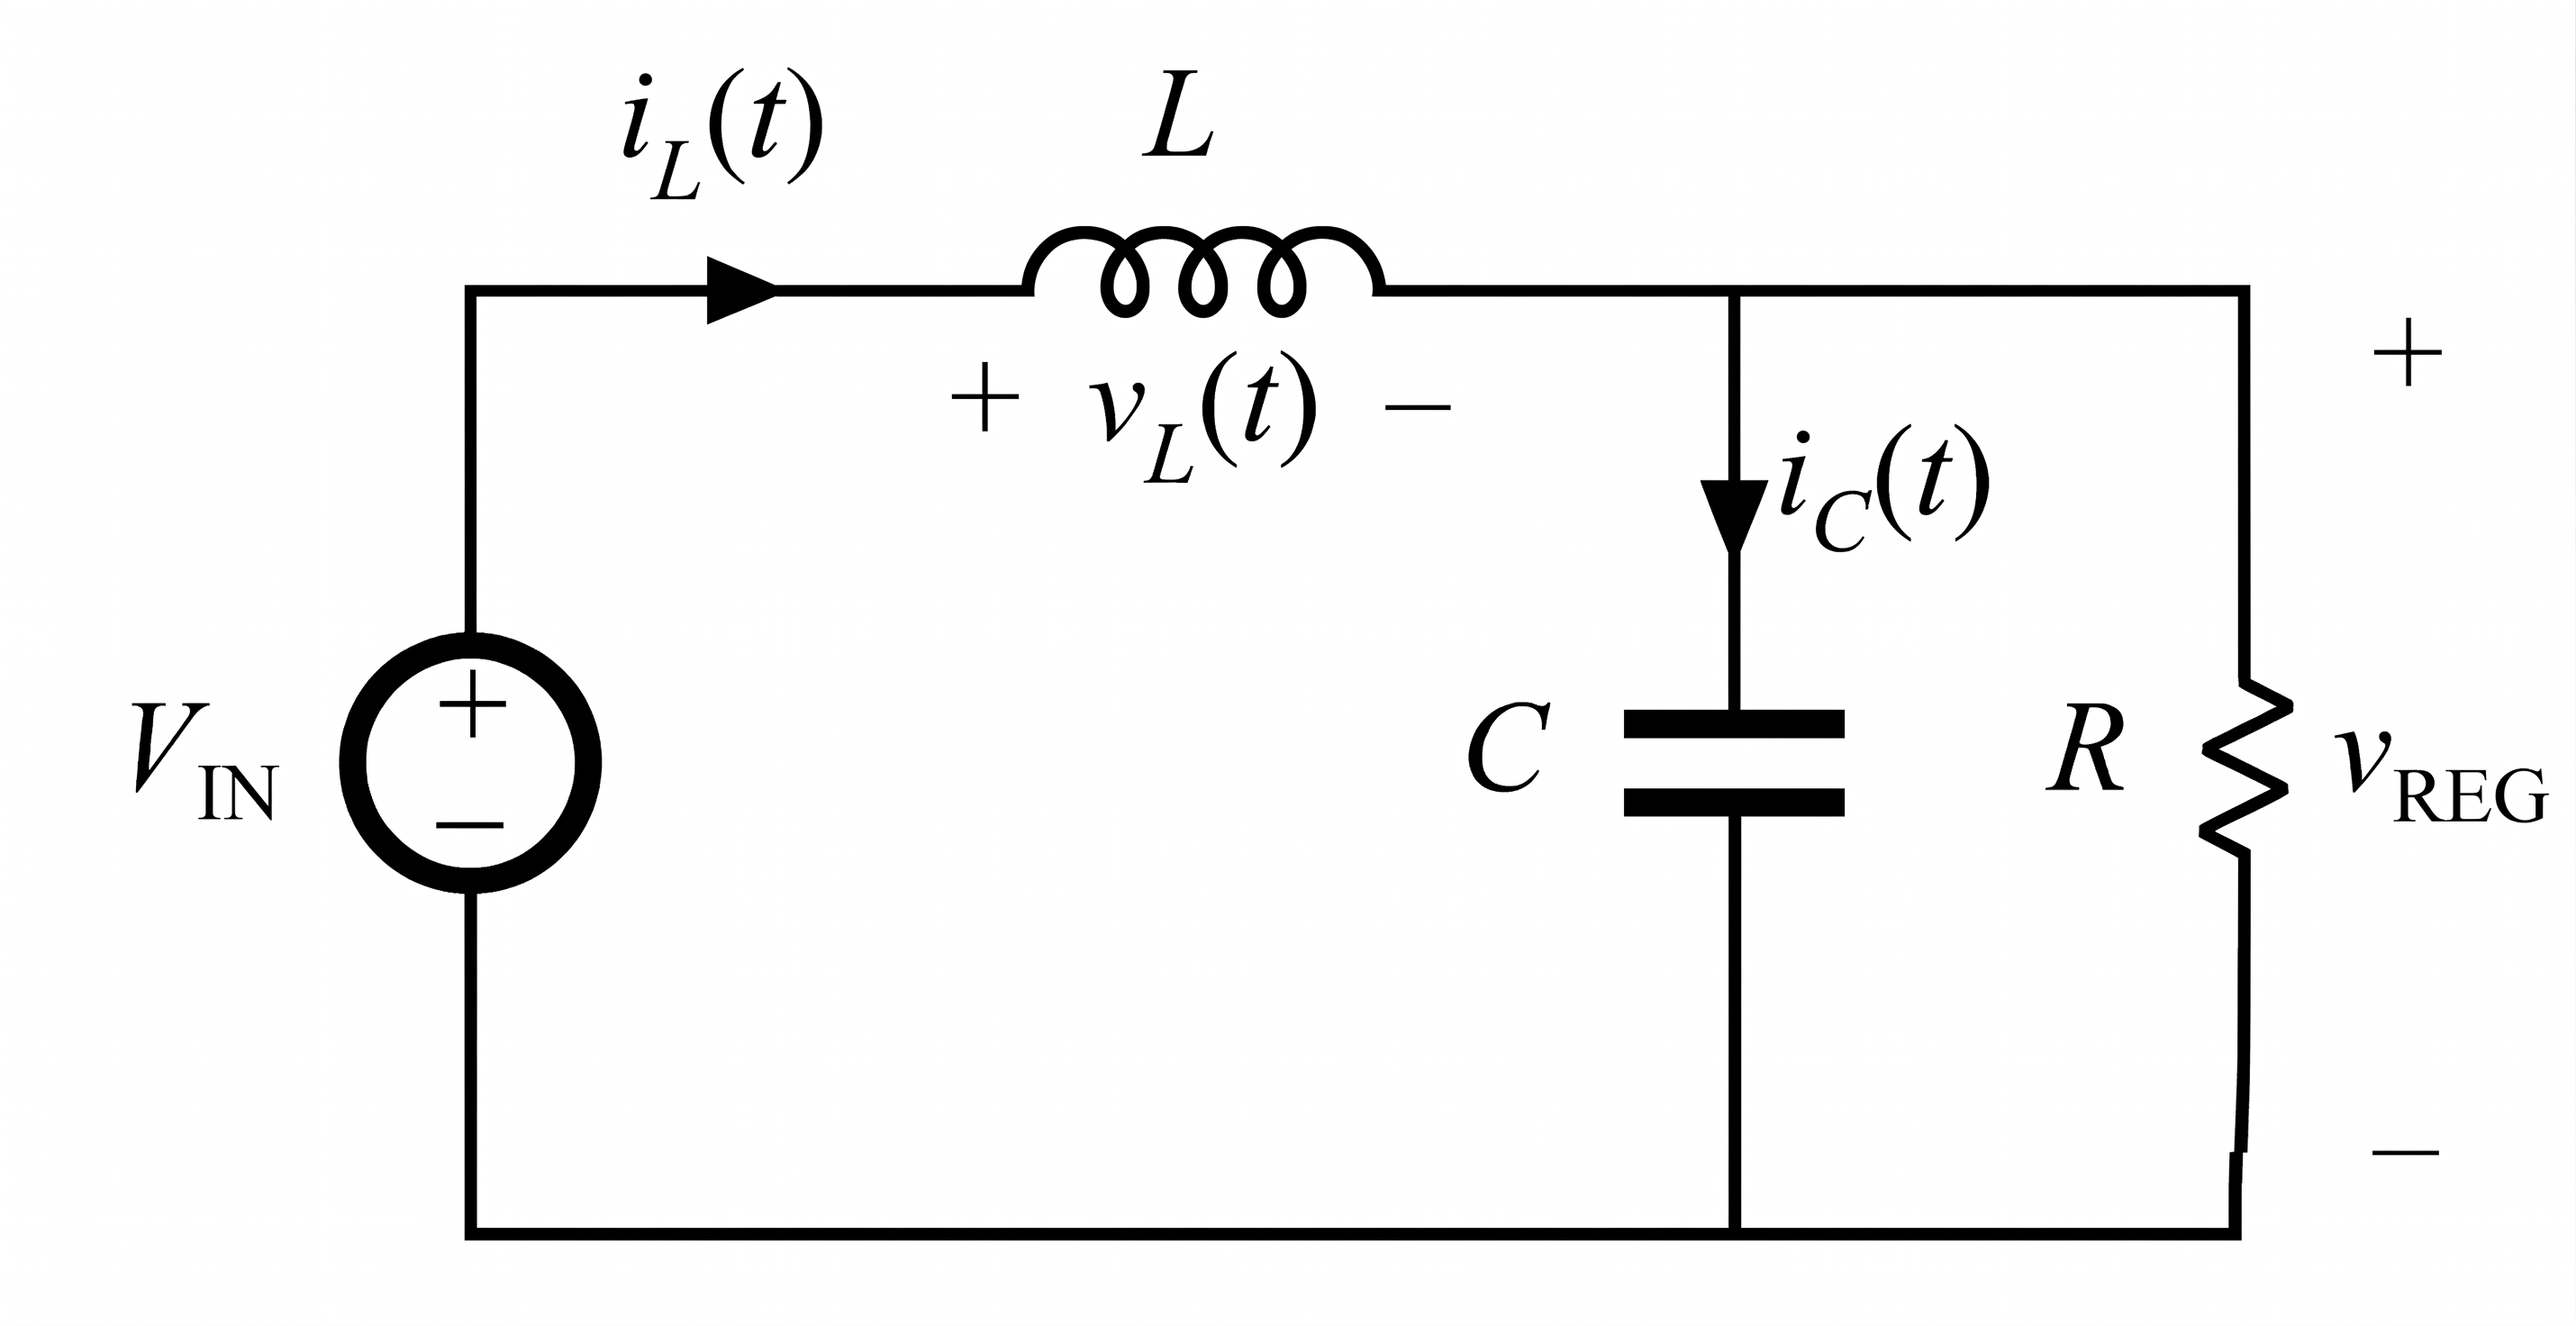
\includegraphics[width=0.65\textwidth]{img/first-position.png}
  \caption{Circuito en posición 1.}
  \label{fig:first-position}
\end{figure}


Aplicando la \textit{small ripple approximation (SRA)},

\begin{equation}
    v_\text{REG}(t) \approx V_\text{REG},
\end{equation}

se obtiene

\begin{equation}
    v_L(t) \approx V_{IN} - V_\text{REG}.
\end{equation}

Como la relación tensión-corriente del inductor está dada por

\begin{equation}
    v_L(t) = L \frac{di_L(t)}{dt},
\end{equation}

la pendiente de la corriente del inductor durante esta posición es

\begin{equation}
    \frac{di_L(t)}{dt} = \frac{V_{IN} - V_\text{REG}}{L}.
\end{equation}

En el \textit{buck converter} se cumple que $V_{IN} > V_\text{REG}$, por lo que la tensión sobre el inductor es positiva. En consecuencia, la corriente $i_L(t)$ crece linealmente durante este intervalo.

La corriente del capacitor se obtiene a partir de la ley de corrientes en el nodo de salida:

\begin{equation}
    i_C(t) = i_L(t) - i_o(t).
\end{equation}

Si la carga se modela mediante una resistencia equivalente $R$, entonces

\begin{equation}
    i_o(t) \approx I_o = \frac{V_\text{REG}}{R}.
\end{equation}

Por lo tanto,

\begin{equation}
    i_C(t) \approx i_L(t) - I_o.
\end{equation}

\subsubsection{Segunda posición: descarga del inductor}

Durante el intervalo

\begin{equation}
    D T_s < t < T_s,
\end{equation}

el nodo de conmutación queda conectado a masa, como se muestra en la fig. \ref{fig:second-position}. En este caso, la tensión aplicada sobre el inductor resulta

\begin{equation}
    v_L(t) = -v_\text{REG}(t).
\end{equation}

\begin{figure}[H]
  \centering
  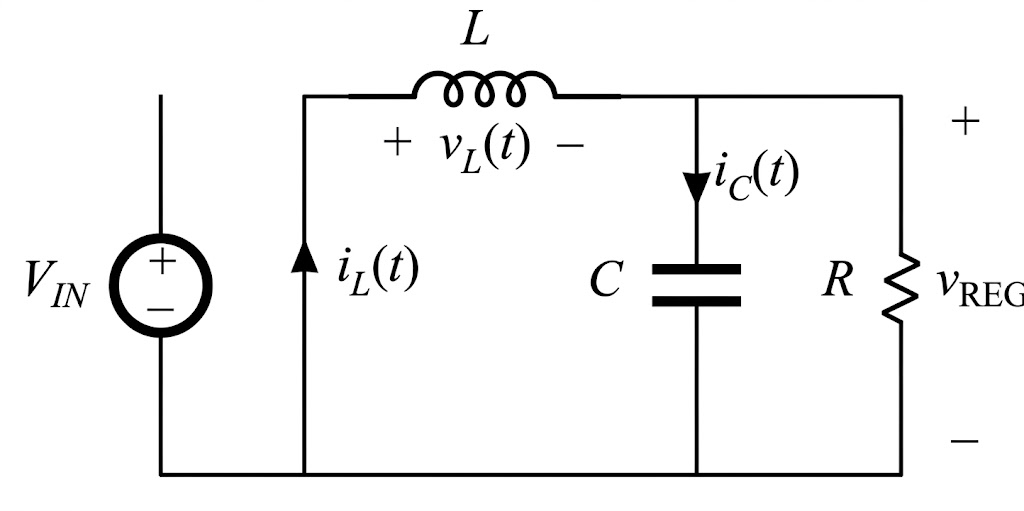
\includegraphics[width=0.65\textwidth]{img/second-position.png}
  \caption{Circuito en posición 2.}
  \label{fig:second-position}
\end{figure}

Aplicando nuevamente la \textit{small ripple approximation (SRA)},

\begin{equation}
    v_L(t) \approx -V_\text{REG}.
\end{equation}

Luego,

\begin{equation}
    \frac{di_L(t)}{dt} = -\frac{V_\text{REG}}{L}.
\end{equation}

La tensión sobre el inductor es negativa, de modo que la corriente $i_L(t)$ decrece linealmente durante este intervalo.

La corriente del capacitor sigue dada por

\begin{equation}
    i_C(t) = i_L(t) - i_o(t),
\end{equation}

y, bajo el modelo resistivo de carga,

\begin{equation}
    i_C(t) \approx i_L(t) - I_o.
\end{equation}

\subsubsection{Interpretación física de los dos estados}

La primera posición puede interpretarse como una etapa de carga del inductor. La entrada entrega energía al circuito, parte de esa energía alimenta a la carga y otra parte queda almacenada en el campo magnético del inductor. Por eso la corriente $i_L(t)$ aumenta.

Cuando el circuito pasa a la segunda posición, la entrada queda desconectada del filtro de salida. Sin embargo, la corriente de un inductor no puede cambiar instantáneamente. Para sostener la circulación de corriente hacia la carga, el inductor invierte la polaridad de su tensión. Esa inversión de $v_L(t)$ es justamente lo que permite que la corriente siga circulando en el mismo sentido, aunque ahora con pendiente negativa.

Por lo tanto, el inductor se carga durante la primera posición y se descarga durante la segunda. En régimen permanente, la energía que gana durante una parte del ciclo debe ser igual a la energía que entrega durante la otra parte. Esta idea se formaliza mediante el \textit{Inductor Volt-Second Balance (IVSB)}.

\subsection{\textit{Inductor Volt-Second Balance}}

En régimen permanente, la corriente del inductor debe repetir su forma de onda ciclo a ciclo. Esto significa que el incremento neto de corriente en un período de conmutación debe ser nulo:

\begin{equation}
    \Delta i_L^{(+)} + \Delta i_L^{(-)} = 0.
\end{equation}

Como la corriente del inductor está relacionada con la tensión por

\begin{equation}
    v_L(t) = L \frac{di_L(t)}{dt},
\end{equation}

la variación de corriente durante un intervalo depende del área de la tensión aplicada sobre el inductor. Por este motivo, pedir que la corriente vuelva al mismo valor al finalizar cada período equivale a pedir que el área neta de $v_L(t)$ en un período sea nula:

\begin{equation}
    \int_0^{T_s} v_L(t)\,dt = 0.
\end{equation}

O, equivalentemente,

\begin{equation}
    \left< v_L(t) \right> = 0.
\end{equation}

Durante la primera posición, de duración $D T_s$, el inductor queda sometido a una tensión positiva:

\begin{equation}
    v_L(t) = V_{IN} - V_o.
\end{equation}

Durante la segunda posición, de duración $(1-D)T_s$, la tensión sobre el inductor toma un valor negativo:

\begin{equation}
    v_L(t) = -V_o.
\end{equation}

Por lo tanto, $v_L(t)$ resulta una onda rectangular de dos niveles, como se muestra en la Fig.~\ref{fig:vl-balance}. El área positiva, asociada al incremento de $i_L(t)$, debe ser igual en módulo al área negativa, asociada a su decremento.

\begin{figure}[H]
  \centering
  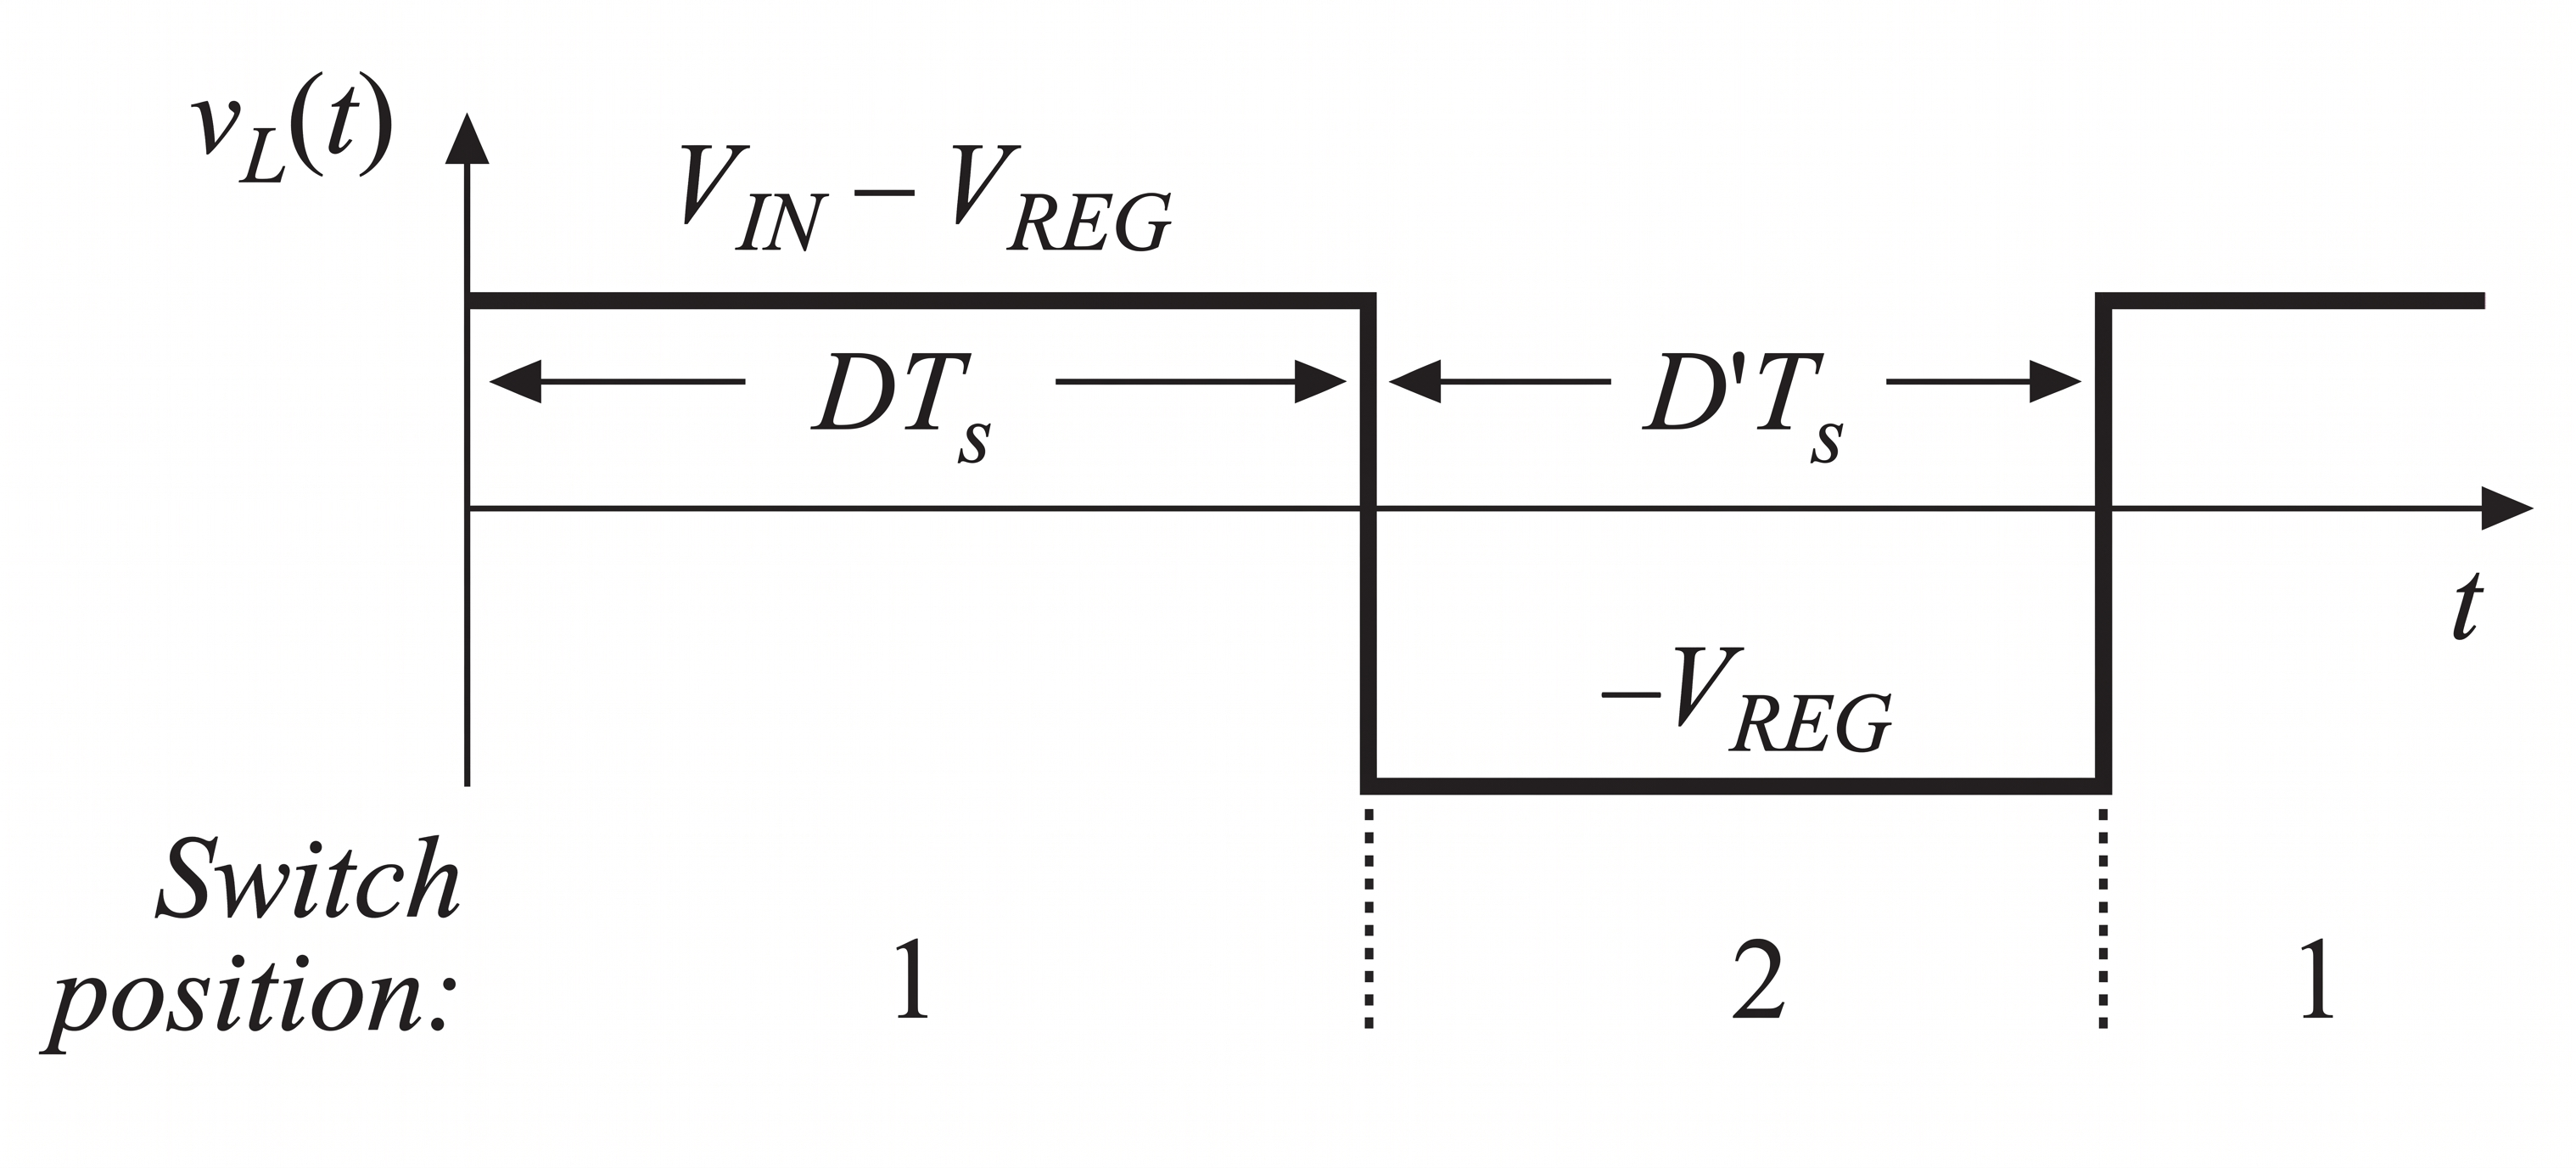
\includegraphics[width=0.5\textwidth]{img/vl-balance.png}
  \caption{Forma de onda ideal de $v_L(t)$ en un período de conmutación. En steady-state, el área positiva durante $D T_s$ debe ser igual en módulo al área negativa durante $(1-D)T_s$.}
  \label{fig:vl-balance}
\end{figure}

Aplicando el \textit{Inductor Volt-Second Balance} al \textit{buck converter}:

\begin{equation}
    (V_{IN}-V_o)D T_s + (-V_o)(1-D)T_s = 0.
\end{equation}

Dividiendo por $T_s$:

\begin{equation}
    D(V_{IN}-V_o) + (1-D)(-V_o) = 0.
\end{equation}

Desarrollando:

\begin{equation}
    D V_{IN} - D V_o - V_o + D V_o = 0.
\end{equation}

Se cancelan los términos $D V_o$:

\begin{equation}
    D V_{IN} - V_o = 0.
\end{equation}

Por lo tanto, la relación de conversión (\textit{conversion ratio} $M(D)$) ideal del \textit{buck} en CCM es

\begin{equation}
    \boxed{M(D)=\frac{V_o}{V_{IN}} = D}
\end{equation}

Para ayudar a visualizar, en la fig. \ref{fig:conversion-ratio} se muestra la relación de conversión del regulador.

\begin{figure}[H]
  \centering
  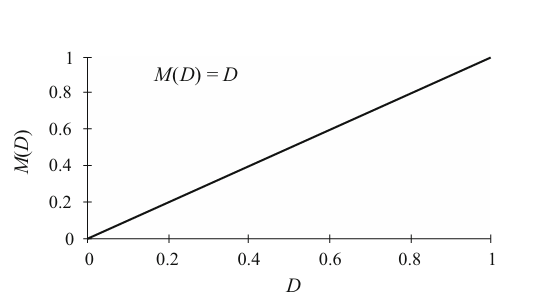
\includegraphics[width=0.5\textwidth]{img/conversion-ratio.png}
  \caption{\textit{Conversion ratio} del \textit{buck converter}.}
  \label{fig:conversion-ratio}
\end{figure}

Equivalentemente, la fórmula anterior se puede escribir cómo

\begin{equation}
    \boxed{V_o = D V_{IN}}.
\end{equation}

Esta ecuación muestra que, en el caso ideal y operando en CCM, la tensión de salida queda determinada directamente por el \textit{duty cycle}. Físicamente, esto tiene sentido: si el nodo de conmutación permanece más tiempo conectado a $V_{IN}$, el valor medio aplicado al filtro aumenta y, por lo tanto, también aumenta la tensión de salida.

\subsection{Ciclo de trabajo requerido}

Para obtener $V_o = V_{REG} = 9.5\ \si{\volt}$, el ciclo de trabajo ideal debe ser

\begin{equation}
    D = \frac{V_o}{V_{IN}}.
\end{equation}

Para la mínima tensión de entrada:

\begin{equation}
    D_{max} = \frac{9.5}{12} = 0.792.
\end{equation}

Para la máxima tensión de entrada:

\begin{equation}
    D_{min} = \frac{9.5}{30} = 0.317.
\end{equation}

Por lo tanto, el rango ideal de operación del PWM es aproximadamente

\begin{equation}
    \boxed{0.317 \leq D \leq 0.792}.
\end{equation}

\subsection{\textit{Capacitor Charge Balance (CCB)}}

En régimen permanente, el capacitor no puede acumular carga neta ciclo a ciclo. Esto implica que la corriente neta que circula por el capacitor durante un período de conmutación debe ser cero:

\begin{equation}
    \Delta Q_C = \int_0^{T_s} i_C(t)\, dt = 0,
\end{equation}

o equivalentemente, que el valor medio de la corriente del capacitor sea nulo:

\begin{equation}
    \left< i_C \right> = 0.
\end{equation}

Dado que la corriente del capacitor es la diferencia entre la corriente del inductor y la corriente de carga:

\begin{equation}
    i_C(t) = i_L(t) - i_o(t),
\end{equation}

se obtiene la condición de balance de carga:

\begin{equation}
    \left< i_L \right> - I_o = 0 \quad \Rightarrow \quad \boxed{\left< i_L \right> = I_o}.
\end{equation}

Es decir, la corriente media del inductor debe ser igual a la corriente media entregada a la carga.

Esta relación es clave para dimensionar el capacitor: cuanto mayor sea la corriente alterna $i_C(t)$, mayor deberá ser $C$ para mantener un rizado de tensión $\Delta V_\text{REG}$ dentro del límite deseado. La misma condición sirve para conectar la corriente del inductor con el \textit{ripple} de salida y, por lo tanto, para justificar conjuntamente los valores de $L$ y $C$.

\subsection{\textit{Ripple} de corriente en el inductor}

Durante un período de conmutación $T_s$, la corriente del inductor $i_L(t)$ varía linealmente en dos intervalos:

\begin{itemize}
    \item \textbf{Intervalo de carga (duración $D T_s$):} el nodo de conmutación está conectado a $V_{IN}$ y la tensión sobre el inductor es positiva
    \begin{equation}
        v_L = V_{IN} - V_\text{REG} \quad \Rightarrow \quad \frac{di_L}{dt} = \frac{V_{IN} - V_\text{REG}}{L}.
    \end{equation}
    La corriente aumenta con pendiente positiva.
    
    \item \textbf{Intervalo de descarga (duración $(1-D) T_s$):} el nodo de conmutación está conectado a tierra y la tensión sobre el inductor es negativa
    \begin{equation}
        v_L = -V_\text{REG} \quad \Rightarrow \quad \frac{di_L}{dt} = -\frac{V_\text{REG}}{L}.
    \end{equation}
    La corriente disminuye con pendiente negativa.
\end{itemize}

Para una mejor compresión, en la fig. \ref{fig:iL-ripple} se aprecia lo explicado anteirormente.

\begin{figure}[H]
  \centering
  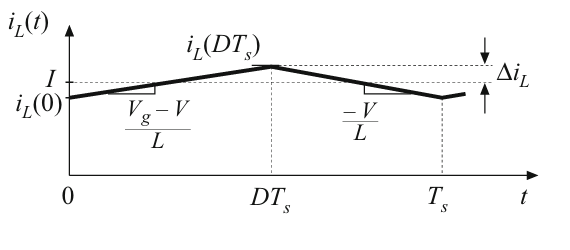
\includegraphics[width=0.6\textwidth]{img/iL-ripple.png}
  \caption{Forma de onda triangular de $i_L(t)$ mostrando el rizado $\Delta i_L$.}
  \label{fig:iL-ripple}
\end{figure}


En régimen permanente, el rizado de corriente $\Delta i_L$ corresponde a la diferencia entre la corriente máxima y mínima, es decir, la altura de un triángulo rectángulo formado por los intervalos de carga y descarga:

\begin{equation}
    \Delta i_L = \frac{(V_{IN}-V_\text{REG})D T_s + V_\text{REG} (1-D) T_s}{2L}.
\end{equation}

Reescribiendo en función del duty cycle $D$ y la frecuencia de conmutación $f_s = 1/T_s$:

\begin{equation}
    \Delta i_L = \frac{V_\text{REG} (1-D)}{2 L f_s}.
\end{equation}

De esta expresión se despeja el valor de la inductancia necesario para limitar el rizado a un valor deseado $\Delta i_L$:

\begin{equation}
    \boxed{L = \frac{V_\text{REG} (1-D)}{2 f_s \Delta i_L}}.
\end{equation}

\textbf{Nota:} el peor caso de rizado se presenta para la menor duty $D_\text{min}$, es decir, para la máxima tensión de entrada $V_{IN,\max}$. Por lo tanto, al dimensionar el inductor se toma:

\begin{equation}
    V_{IN,\max} = 30\ \si{\volt}, \quad D_\text{min} = 0.317.
\end{equation}

Cabe aclarar que en este informe, se define \(\Delta i_L\) como la desviación máxima de la corriente respecto de su valor medio. Por lo tanto, el rizado pico a pico de la corriente del inductor resulta igual a \(2\Delta i_L\).

\subsection{Condición de conducción continua}

El análisis desarrollado en las secciones anteriores se realizó suponiendo operación en \textit{Continuous Conduction Mode} (CCM), es decir, considerando que la corriente del inductor no es nula durante el período de conmutación.

Por este motivo, el dimensionamiento preliminar del inductor se realizó buscando que el regulador opere en CCM para todo el rango previsto de funcionamiento. En particular, se seleccionó el valor de inductancia de forma tal que el \textit{ripple} de corriente $\Delta i_L$ sea menor que la corriente mínima de carga esperada, evitando así que la corriente del inductor alcance el cero.

Esta hipótesis permite utilizar las relaciones ideales derivadas previamente, como

\begin{equation}
\frac{V_o}{V_{IN}} = D,
\end{equation}

además de simplificar el análisis del convertidor al mantener una dinámica lineal por tramos.

En caso de que la corriente del inductor se anule durante parte del período, el convertidor pasaría a operar en \textit{Discontinuous Conduction Mode} (DCM), situación en la cual las expresiones ideales obtenidas dejan de ser válidas y la relación de conversión depende además de la carga y de la inductancia.

\subsection{Selección preliminar del inductor}

\label{sec:inductor}

Dado que la corriente mínima en el inductor será de aproximadamente 100$\,$mA, su \textit{ripple} debe ser menor para que la \textit{buck} no opere en modo crítico. 

Se elige un ripple $\Delta i_L = 70\,$mA para tener un margen de seguridad y garantizar siempre el modo continuo. Teniendo en cuenta que $V_\text{REG} = 9,5\,$V, $f_s = 130\,$kHz y $D_\text{min} = 0,317$, se obtine una inductancia 

\[
L = 356,5\,\mu\text{H}\,.
\]

Más adelante, hay una sección hecha especialmene enfocada en el diseño del inductor.

\subsection{\textit{Ripple} de tensión de salida}

Bajo la hipótesis de \textit{small ripple}, la corriente del inductor puede aproximarse mediante una señal triangular centrada en su valor medio. Como el valor medio de la corriente del capacitor es nulo, la componente alterna de la corriente del inductor circula a través del capacitor de salida.

Por lo tanto, la corriente del capacitor puede aproximarse como una onda triangular de amplitud pico

\begin{equation}
    I_{C,p}=\frac{\Delta i_L}{2}.
\end{equation}

La variación de tensión en el capacitor está dada por

\begin{equation}
    i_C(t)=C\frac{dv_C(t)}{dt}.
\end{equation}

Durante la mitad de un semiciclo, la carga transferida al capacitor corresponde al área de un triángulo de base $T_s/2$ y altura $\Delta i_L/2$:

\begin{equation}
    \Delta Q=
    \frac{1}{2}
    \left(\frac{T_s}{2}\right)
    \left(\Delta i_L}\right)
    =
    \frac{\Delta i_L T_s}{4}.
\end{equation}

Como la variación de tensión de un capacitor verifica

\begin{equation}
    \Delta V_o=\frac{\Delta Q}{C},
\end{equation}

se obtiene el \textit{ripple} pico a pico de salida

\begin{equation}
    \boxed{
    \Delta V_o=
    \frac{\Delta i_L}
         {4 C f_s}
    }.
\end{equation}

Despejando el valor mínimo de capacidad necesario para limitar el \textit{ripple} a un valor especificado,

\begin{equation}
    \boxed{
    C \ge
    \frac{\Delta i_L}
         {4 f_s \Delta V_o}
    }.
\end{equation}

Finalmente, se desea limitar el \textit{ripple} de tensión de salida a un valor máximo de
\[
\Delta V_o = 200\,\text{mV}.
\]

Considerando el \textit{ripple} de corriente previamente adoptado para el inductor,
\[
\Delta i_L = 70\,\text{mA},
\]
y una frecuencia de conmutación de
\[
f_s = 130\,\text{kHz},
\]
la capacidad mínima necesaria resulta

\[
C \ge
\frac{\Delta i_L}{4f_s\Delta V_o}
=
0.673\,\mu\text{F}.
\]

Por lo tanto, cualquier capacitor de valor superior a $0.68\,\mu\text{F}$ cumple con la especificación de \textit{ripple} en el modelo ideal. En la práctica, se seleccionará un valor mayor para compensar los efectos de ESR, tolerancias de fabricación y variaciones de los parámetros de los componentes.

\subsubsection{Efecto de la ESR del capacitor}

En un capacitor real, la resistencia serie equivalente introduce una componente adicional de rizado dada aproximadamente por

\begin{equation}
    \Delta v_{ESR} \approx \Delta i_L \cdot ESR.
\end{equation}

Por lo tanto, el rizado total de salida puede estimarse como la suma de la contribución capacitiva y la contribución resistiva:

\begin{equation}
    \Delta v_o \approx \frac{\Delta i_L}{4 C f_s} + \Delta i_L \cdot ESR.
\end{equation}

Esto muestra que no alcanza con elegir un valor grande de capacidad: también es importante seleccionar capacitores con baja ESR, especialmente en fuentes conmutadas.

Debido a que la elección del tamaño del capacitor fue resultado de un análisis que no contempla las parasíticas presentes en una implementación real, tales como la resistencia serie equivalente (ESR) y la inductancia serie equivalente (ESL) de los componentes, además de las inductancias y capacidades distribuidas del circuito impreso, se optó por adoptar un capacitor de $1,\mu\text{F}$ como valor de diseño.

Por otra parte, una práctica habitual en fuentes conmutadas consiste en utilizar varios capacitores en paralelo. Esto permite reducir la resistencia serie equivalente (ESR) y la inductancia serie equivalente (ESL) vistas desde la salida del regulador.


\subsection{Modelo de carga equivalente del LDO}

El \textit{buck} no alimenta directamente una carga resistiva pura, sino la entrada de un regulador lineal LDO. Sin embargo, para realizar el análisis inicial del regulador se puede representar al LDO mediante una resistencia equivalente asociada al punto de operación:

\begin{equation}
    R_{eq} = \frac{V_{REG}}{I_{REG}}.
\end{equation}

Para la corriente máxima de salida:

\begin{equation}
    R_{eq,min} = \frac{9.5}{1.5} = 6.33\ \si{\ohm}.
\end{equation}

Para una corriente de carga de $100\ \si{\milli\ampere}$:

\begin{equation}
    R_{eq,max} = \frac{9.5}{0.1} = 95\ \si{\ohm}.
\end{equation}

Este modelo permite aplicar el análisis clásico del \textit{buck} en una primera etapa. Sin embargo, debe recordarse que el LDO no es estrictamente una resistencia: su corriente de entrada depende de la corriente de salida, de su corriente de polarización interna y de las condiciones de operación. Por eso, el modelo resistivo debe entenderse como una aproximación útil para el diseño preliminar y la simulación inicial.

\subsection{Resumen de diseño ideal}

A partir del análisis ideal del convertidor \textit{buck} en conducción continua se obtuvieron las siguientes expresiones principales:

\begin{equation}
    \frac{V_o}{V_{IN}} = D
\end{equation}

\begin{equation}
    \Delta i_L = \frac{V_o(1-D)}{L f_s}
\end{equation}

\begin{equation}
    L = \frac{V_o(1-D)}{2 \Delta i_L f_s}
\end{equation}

\begin{equation}
    \Delta v_o \approx \frac{\Delta i_L}{4 C f_s}
\end{equation}

\begin{equation}
    C \geq \frac{\Delta i_L}{4 f_s \Delta v_o}.
\end{equation}

Con los criterios adoptados para el diseño preliminar:

\begin{itemize}
    \item $V_{IN}=12\ \si{\volt}$ a $30\ \si{\volt}$.
    \item $V_o=V_{REG}=9.5\ \si{\volt}$.
    \item $f_s=130\ \si{\kilo\hertz}$.
    \item $I_{o,max}=1.5\ \si{\ampere}$.
    \item $\Delta i_L=\SI{70}{\milli\ampere}$.
    \item $\Delta v_o=200\ \si{\milli\volt}$.
\end{itemize}

se obtiene:

\begin{equation}
    \boxed{ L = 356,5\,\mu\text{H}\,.}
\end{equation}

y

\begin{equation}
    \boxed{C = 1\ \si{\micro\farad}}.
\end{equation}

Estos valores constituyen una primera aproximación ideal, que luego deberá verificarse mediante simulación considerando MOSFETs reales, tiempos muertos, resistencia serie del inductor, ESR del capacitor y pérdidas de conmutación.

\subsection{Implementación de los interruptores de potencia}

En la implementación práctica del convertidor \textit{buck}, los interruptores ideales fueron reemplazados por dos MOSFETs de potencia IRFZ44N configurados como \textit{synchronous rectifiers}, tal como se muestra en la Figura \ref{fig:rectificador-sincrono}.

\begin{figure}[H]
\centering
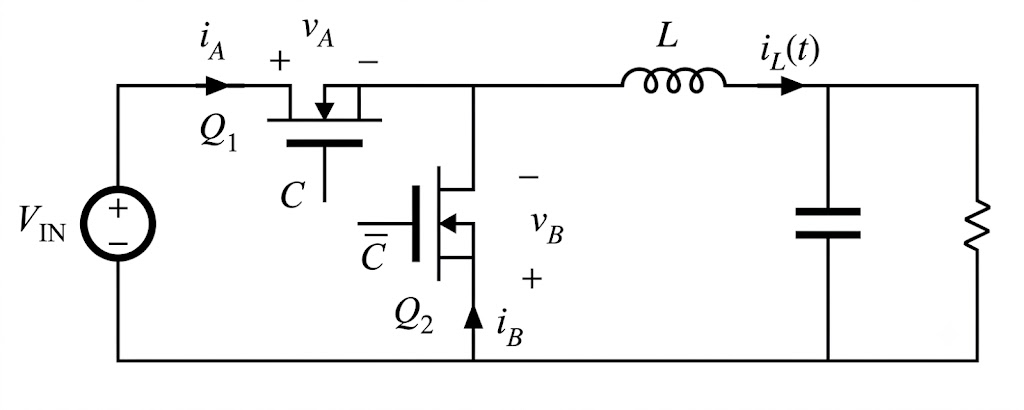
\includegraphics[width=0.6\textwidth]{img/rectificador-sincrono.jpg}
\caption{Etapa de potencia implementada mediante rectificación síncrona.}
\label{fig:rectificador-sincrono}
\end{figure}

Las compuertas de ambos MOSFETs son excitadas mediante señales PWM complementarias. Adicionalmente, se introduce un pequeño \textit{dead time} entre las transiciones de encendido y apagado para evitar la conducción simultánea de ambos dispositivos (\textit{shoot-through}), situación que produciría una corriente elevada entre la alimentación y masa.

Se optó por utilizar una topología de rectificación síncrona en lugar de la implementación clásica basada en un MOSFET y un diodo rápido. La principal ventaja de esta configuración es la reducción de las pérdidas de conducción.

En una implementación convencional, durante el intervalo donde el diodo está encendido, la caída de tensión es aproximadamente constante. Considerando una caída típica de \SI{0.2}{\volt} para diodos rápidos y una corriente máxima de carga de \SI{1.5}{\ampere}, las pérdidas asociadas serían del orden de

\[
P_D \approx V_F I \approx 0.3,\text{W}.
\]

En cambio, utilizando un MOSFET como rectificador síncrono, las pérdidas de conducción vienen dadas por

\[
P_{MOS} \approx I^2 R_{DS(on)}.
\]

Para el IRFZ44N, cuya resistencia de conducción es del orden de \SI{22}{\milli\ohm}, se obtiene

\[
P_{MOS} \approx (1.5)^2 \cdot 22,\text{m}\Omega
\approx 50,\text{mW}.
\]

Por lo tanto, la utilización de rectificación síncrona reduce significativamente las pérdidas de potencia y mejora la eficiencia global del regulador.

El dispositivo seleccionado fue el MOSFET IRFZ44N, un transistor de potencia de canal N basado en tecnología TrenchMOS. Su elección se fundamenta en las siguientes características:

\begin{itemize}
\item $V_{DS\text{max}}=\SI{55}{\volt}$ , ampliamente superior a la tensión máxima de entrada del regulador ($\SI{30}{\volt}$).

\item $I_{D\text{max}} = \SI{49}{\ampere}$, muy por encima de la corriente máxima prevista en la aplicación ($\SI{1.5}{\ampere}$).

\item Baja resistencia de conducción, con un valor típico de \(R_{DS(on)}\) inferior a $\SI{22}{\milli\ohm}$, lo que minimiza las pérdidas por conducción.

\item Elevada capacidad de disipación de potencia ($\SI{110}{\watt}$) y encapsulado TO-220, facilitando su utilización sin exigir condiciones térmicas extremas.

\item Tiempos de conmutación reducidos y bajas capacitancias parásitas, características adecuadas para la frecuencia de operación seleccionada ($\SI{130}{\kilo\hertz}$).

\end{itemize}

Estas características proporcionan amplios márgenes eléctricos y térmicos para la aplicación, permitiendo implementar una etapa de potencia robusta y eficiente.

\section{Capacitor de entrada}

En un convertidor \textit{buck}, el capacitor de entrada $C_E$ que se muestra en la Figura \ref{fig:capentrada} se coloca en paralelo con la fuente para suministrar localmente la corriente pulsante demandada por el interruptor. Cuando el transistor conmuta, la corriente absorbida desde la entrada no es continua, sino que presenta pulsos de alta frecuencia. Si no existiera este capacitor, dichos pulsos deberían ser entregados directamente por la fuente a través de los conductores y pistas del circuito, generando caídas de tensión indeseadas debido a las resistencias e inductancias parásitas.

\begin{figure}[H]
    \centering
    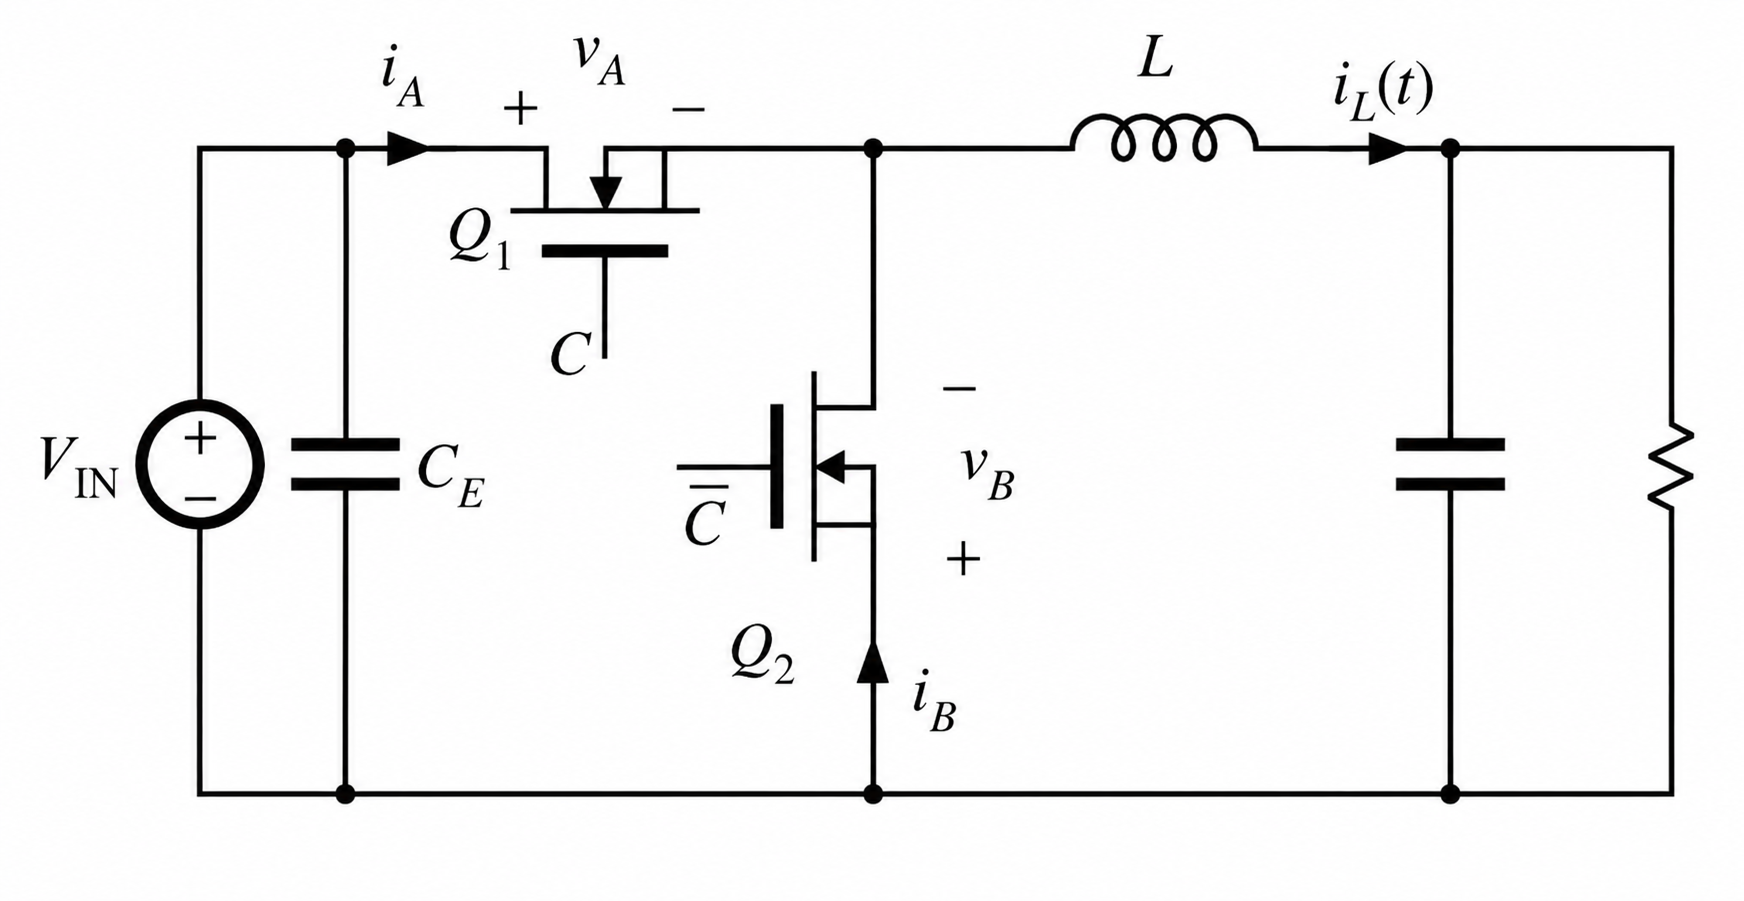
\includegraphics[width=0.8\textwidth]{img/capentrada.png}
    \caption{Fuente conmutada final a lazo abierto.}
    \label{fig:capentrada}
\end{figure}

Además, $C_E$ reduce el \textit{ripple} de tensión en la entrada. Durante los intervalos en que el transistor conduce, el capacitor entrega parte de la energía requerida por el inductor y la carga; cuando el transistor se apaga, el capacitor se recarga desde la fuente. De esta manera, la tensión de entrada permanece prácticamente constante, mejorando el funcionamiento del convertidor.

Por otra parte, el capacitor de entrada ayuda a disminuir las interferencias electromagnéticas (EMC) producidas por las rápidas variaciones de corriente asociadas a la conmutación. Al proporcionar un camino de baja impedancia para las componentes de alta frecuencia, evita que estas perturbaciones se propaguen hacia la fuente de alimentación y al resto del sistema.

En la práctica, el capacitor de entrada suele implementarse mediante la conexión en paralelo de dos tipos de capacitores. Por un lado, se emplea un capacitor electrolítico o de polímero de varios $\mu$F a cientos de $\mu$F cuya función principal es almacenar energía y reducir las variaciones de tensión de baja frecuencia. Por otro lado, se utiliza un capacitor cerámico de baja ESR, típicamente entre $100\,\mathrm{nF}$ y $10\,\mu\mathrm{F}$, ubicado físicamente muy cerca del MOSFET. Este último proporciona un camino de baja impedancia para las componentes de alta frecuencia de la corriente de conmutación, reduciendo el ruido y las interferencias electromagnéticas.

\section{Diseño del inductor}

Se desea diseñar un inductor como el que se muestra en la Figura \ref{fig:inductor}, donde $i(t) = i_L$ es la corriente que circula por el inductor, $v(t) = v_L$ es su tensión, $n$ es la cantidad de espiras que lo conforman, $\Phi$ es el flujo magnético, $\mathcal{R}_c$ es la reluctania del núcleo, $\mathcal{R}_g$ es la reluctancia de la banda de aire y $\mathcal{F}$ es la fuerza magnetomotríz (f.f.m).

\begin{figure}[H]
    \centering
    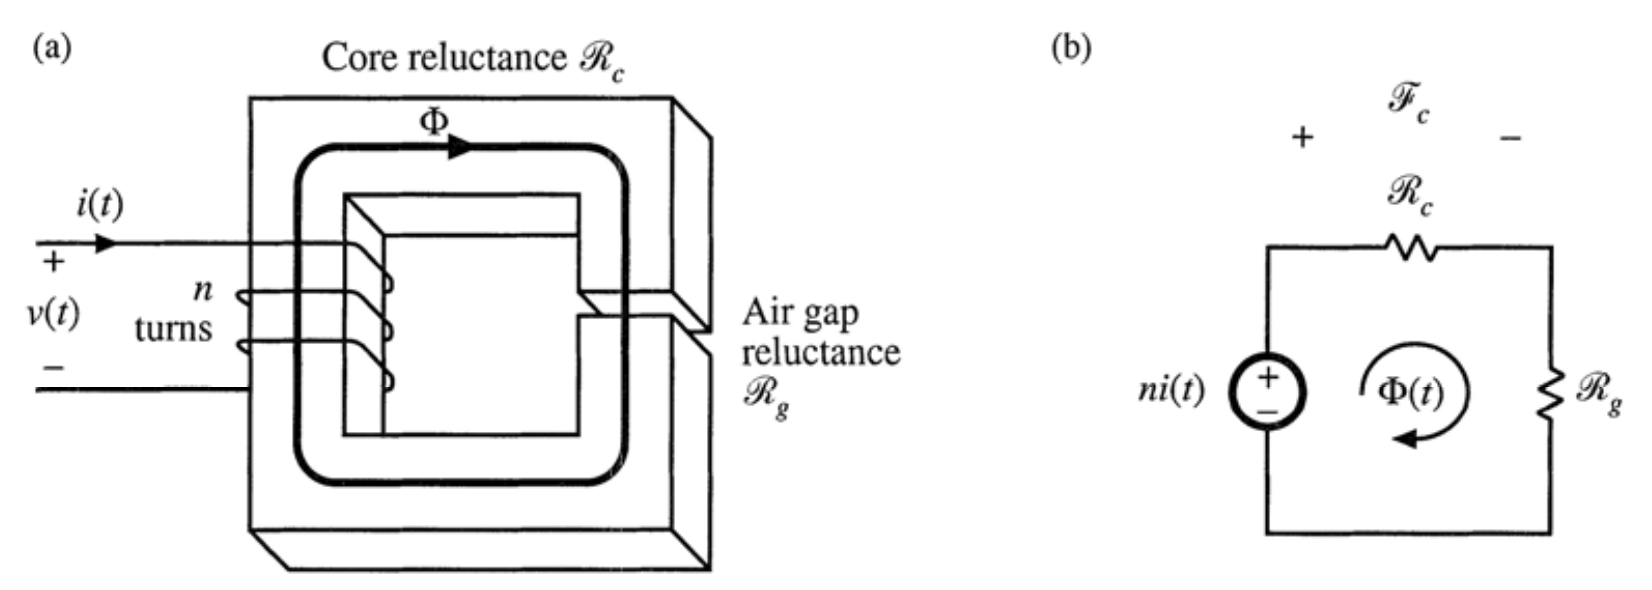
\includegraphics[width=0.8\textwidth]{img/inductor.png}
    \caption{Inductor: (a) estructura, (b) circuito magnético modelado.}
    \label{fig:inductor}
\end{figure}

Sean $\ell_c$, $\ell_g$, $A_c$, $\mu_c$ y $\mu_0$ la longitud media del camino magnético en el núcleo, la longitud del entrehierro, la sección del núcleo, la permeabilidad del núcleo y la permeabilidad del vacío, respectivamente. Entonces, las reluctancias verifican

\[
\mathcal{R}_c = \frac{\ell_c}{\mu_c A_c}; \quad\quad \mathcal{R}_g = \frac{\ell_g}{\mu_0 A_c};    
\]

la f.f.m verifica 

\[
\mathcal{F} = n i_L = \Phi (\mathcal{R}_c + \mathcal{R}_g)\,.    
\]

Como generalmente $\mathcal{R}_c \ll \mathcal{R}_g$, etonces $n i_L \approx \Phi \mathcal{R}_g$. Siendo $B$ el campo magnético, se tiene que $\Phi = B A_c$, por lo que $n i_L = B A_c \mathcal{R}_g$.

Teniendo en cuenta la corriente máxima que circula por el inductor $I_L^\text{max}$ y el campo magnético máximo que soparta $B_\text{max}$, se obtiene

\begin{equation}
n I_L^\text{max} = B_\text{max} A_c \mathcal{R}_g = B_\text{max} \frac{\ell_g}{\mu_0}\,.  
\label{eq:ffm}
\end{equation}

Sea $L$ la inductancia del inductor y $\lambda$ su flujo concatenado tal que $\lambda = n\Phi$. Entonces, por definición 

\begin{equation}
L = \frac{\lambda}{i_L} = \frac{n\Phi}{i_L} = \frac{n^2}{\mathcal{R}_g} = \frac{\mu_0 A_c n^2}{\ell_g}\,.
\label{eq:inductancia}
\end{equation}

Sea $A_W$ la sección del devanado sin aislación y $W_A$ el área de la ventana del núcleo. Entonces, el área de cobre en la ventana es $n A_W$. Definiendo $K_u$ como el factor de utilización de ventana o factor de llenado se tiene que 

\begin{equation}
K_u W_A \ge n A_W\,.
\label{eq:ventana}
\end{equation}

Sea $\ell_b$ la longitud del alambre y MLT la longitud media por espira tal que $\ell_b = n (\text{MLT})$. La resistencia equivalente $R$ del inductor se puede calcular teniendo en cuenta la resistividad del material (cobre en este caso) $\rho_\text{Cu}$ como

\begin{equation}
R = \rho_\text{Cu} \frac{\ell_b}{A_W} = \rho_\text{Cu} \frac{n (\text{MLT})}{A_W}\,.
\label{eq:resistencia}
\end{equation}

De las Ecuaciones \ref{eq:ffm}, \ref{eq:inductancia}, \ref{eq:ventana} y \ref{eq:resistencia} se obtiene la siguiente desigualdad

\[
K_g = \frac{A_c^2 W_A}{\text{MLT}} \ge \frac{\rho_\text{Cu} (L I_L^\text{max})^2}{B_\text{max}^2 R K_u}\,,   
\]

donde $K_g$ es la constante geométrica del núcleo, que tiene unidades de longitud a la quinta.

Por lo tanto, utilizando el método de Erickson, los pasos para calcular el diseño del inductor son los siguientes.

\begin{enumerate}
    \item Resistencia máxima: \[R_\text{max} = \frac{P_\text{Cu}^\text{max}}{I_L^\text{max}}\,.\]
    \item Constante geométrica del núcleo: \[K_g \ge \frac{\rho_\text{Cu}(L I_L^\text{max})^2}{B_\text{max}^2 R K_u}\,.\]
    \item Longitud del entrehierro: \[\ell_g = \frac{\mu_0 L (I_L^\text{max})^2}{B_\text{max}^2 A_c}\,.\]
    \item Número de espiras: \[n = \left\lceil \frac{L I_L^\text{max}}{B_\text{max}A_c} \right\rceil\,.\]
    \item Sección del devanado: \[A_W \le \frac{K_u W_A}{n}\,.\]
    \item Resistencia equivalente: \[R = \frac{\rho_\text{Cu}n (\text{MLT})}{A_W}\,.\]
    \item Longitud del alambre: \[\ell_b = n (\text{MLT})\,.\]
\end{enumerate}

La corriente del inductor es prácticamente la misma que la de la carga de la \textit{buck} (porque el capacitor en régimen permanente funciona como un circuito abierto). Se observó que la corriente de entrada del LDO se pierde casi completamente en su carga (el amplificador de error y las cargas activas se llevan decenas de mA), por lo que las corrientes máxima y mínima en el inductor van a ser aproximadamente igual a las corrientes máxima y mínima en la carga del LDO. Por la foldback, la carga soporta como mucho 1,5 A y como la carga mínima es 50$\,\Omega$, la corriente mínima es 100 mA.

Se especifica una potencia disipada por el cobre máxima de 1 W, por lo que la resistencia máxima será $R_\text{max} = 390\,\mathrm{m\Omega}$.

Como se seleccionó en la Sección \ref{sec:inductor}, se tiene $L = 356,4\,\mathrm{\mu H}$. A temperatura ambiente, la resistividad del cobre es de $1,724 \cdot 10^{-6}\sfrac{\Omega}{\text{cm}}$. Se escoge $B_\text{max} = 0,3\,$T y $K_u = 0,33$, valores típicos. De esta forma, se obtiene una constante geométrica $K_g \ge 4,84 \cdot 10^{-3} \,\mathrm{cm^5}$. Los núcleos que verifican son los EE22, 30, 40, 50, 60, etc. En la Tabla \ref{tab:nucleos_EE} se observan los parámetros geométricos para los primeros cinco núcleos. Asimismo, en la Tabla \ref{tab:parametros_EE} se observan los parámetros de diseño del inductor según el núcleo.

\begin{table}[h]
\centering
\begin{tabular}{|c|c|c|c|c|}
\hline
\textbf{Núcleo} &
\textbf{$K_g$ [cm$^5$]} &
\textbf{$A_c$ [cm$^2$]} &
\textbf{$W_A$ [cm$^2$]} &
\textbf{MLT [cm]} \\
\hline
EE22 & $8,26\cdot10^{-3}$ & 0,41 & 0,196 & 3,99 \\
EE30 & $85,7\cdot10^{-3}$ & 1,09 & 0,476 & 6,60 \\
EE40 & 0,209 & 1,27 & 1,10 & 8,50 \\
EE50 & 0,909 & 2,26 & 1,78 & 10,0 \\
EE60 & 1,38 & 2,47 & 2,89 & 12,8 \\
\hline
\end{tabular}
\caption{Parámetros geométricos de núcleos EE.}
\label{tab:nucleos_EE}
\end{table}

\begin{table}[h]
\centering
\begin{tabular}{|c|c|c|c|c|}
\hline
\textbf{Núcleo} &
\textbf{$l_g$ [mm]} &
\textbf{$n$ [-]} &
\textbf{$A_w$ [cm$^2$]} &
\textbf{$l_b$ [cm]} \\
\hline
EE22 & 0,31 & 47 & $\leq 1,38\cdot10^{-3}$ & 187,53 \\
EE30 & 0,12 & 18 & $\leq 8,73\cdot10^{-3}$ & 118,8 \\
EE40 & 0,10 & 15 & $\leq 24,20\cdot10^{-3}$ & 127,5 \\
EE50 & 0,06 & 9  & $\leq 65,27\cdot10^{-3}$ & 90,0 \\
EE60 & 0,05 & 8  & $\leq 119,21\cdot10^{-3}$ & 102,4 \\
\hline
\end{tabular}
\caption{Parámetros de diseño para los distintos núcleos EE.}
\label{tab:parametros_EE}
\end{table}

Para todos los núcleos se presenta una resistencia equivalente menor a la máxima.

En función del núcleo elegido, la sección del devanado será distinta. Por ejemplo, para el nucleo EE22 se necesitará un alambre AWG\#26 o superior.

En función de la disponibilidad en el mercado, para el próximo \textit{checkpoint} se escogerá una configuración.


\section{Diseño del PCB del \textit{buck converter}}

\begin{figure}[H]
    \centering
    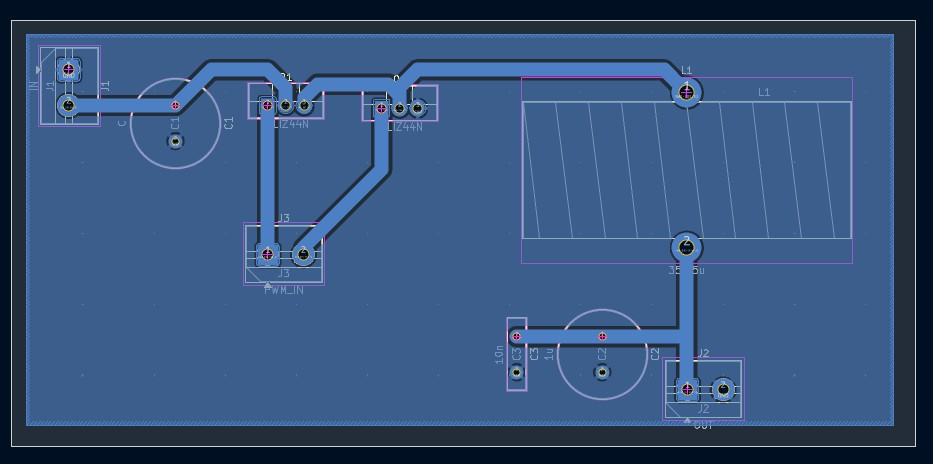
\includegraphics[width=0.8\textwidth]{img/buck PCB.jpg}
    \caption{PCB del \textit{buck converter}}
    \label{fig:pcb buck}
\end{figure}

\begin{figure}[H]
    \centering
    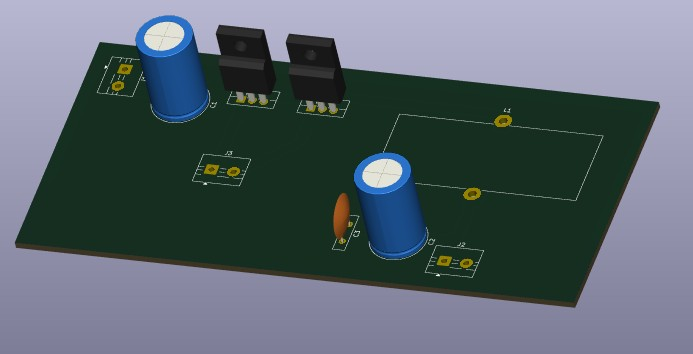
\includegraphics[width=0.8\textwidth]{img/buck PCB3D.jpg}
    \caption{PCB del \textit{buck converter}}
    \label{fig:pcb3d buck}
\end{figure}


Como última etapa de este informe, se diseñó el PCB de la fuente \textit{buck} a lazo abierto. Se procuró utilizar pistas cortas y anchas, minimizando posibles interferencias electromagnéticas y asi como efectos reactivos de las pistas. 

\section{Conclusiones}

Se diseñó e implemento un generador de puslos PWM de manera satifactoria. La frecuencia de las oscilaciones resutló ser de $f = \SI{118}{\kilo \hertz}$.

El análisis hecho en la Sección 2.1, si bien de validez limitada, permitió entender cómo las distintas variables del circuito afectan a las señales generadas. 

También se desarrolló el diseño preliminar de una fuente \textit{buck} a lazo abierto para obtener una tensión intermedia de aproximadamente $\SI{9.5}{\volt}$ a partir de una entrada variable entre $\SI{12}{\volt}$ y $\SI{30}{\volt}$. A partir del modelo ideal en régimen permanente y en conducción continua, se obtuvo la relación entre el ciclo de trabajo y la tensión de salida, y se dimensionaron los componentes principales considerando las condiciones más exigentes de operación.

El análisis de \textit{ripple} permitió seleccionar una inductancia de $\SI{356.4}{\micro\henry}$ y verificar que el convertidor pueda mantenerse en CCM dentro del rango de carga especificado. Además, se estudiaron las solicitaciones eléctricas sobre el MOSFET, el diodo, el capacitor de salida y el capacitor de entrada, lo que permitió justificar la elección de componentes con márgenes adecuados de tensión, corriente y potencia.

Finalmente, se aplicó el método de Erickson para el diseño del inductor, obteniéndose una constante geométrica mínima y comparando distintas alternativas de núcleos EE. Si bien la selección definitiva queda sujeta a la disponibilidad comercial y a la etapa experimental del próximo \textit{checkpoint}, los resultados obtenidos muestran que el diseño propuesto es técnicamente viable y constituye una base consistente para la implementación física del regulador.


\section{Referencias}

[1] P. R. Gray, P. J. Hurst, S. H. Lewis y R. G. Meyer, \textit{Analysis and Design of Analog Integrated Circuits}. Hoboken, NJ: Wiley, 5ta ed., 2009.

[2] STMicroelectronics, ``TIP32C: Power transistor.'', 2006.

[3] Texas Instruments, ``TL431, TL432: Precision Programmable Reference.'', 2025.

[4] ON Semiconductor, ``BC556B, BC557A, B, C, BC558B: Amplifier transistors (PNP Silicon).'', 2007.

[5] Fairchild Semiconductor, ``BC547, BC547A, BC547B, BC547C: NPN General Purpose Amplifier.'', 1997.

[6] Semiconductores y Componentes, ``Disipadores.'', s.f.

[7] Texas Instruments, ``How to Properly Configure Unused Operational Amplifiers.'', SBOA204A, rev. Sept. 2018.

[8] Texas Instruments, ``LM158, LM258, LM2904, LM358: Industry-Standard Dual Operational Amplifiers.'', SLOS068AB, rev. Oct. 2024.

[9] Semiconductores y Componentes, ''78XX 3-Terminal 1A Positive Voltage Regulator''

[9] Texas Instruments, ''LM393B, LM2903B, LM193, LM293, LM393 and LM2903 Dual Comparators'', 1974, rev. 2025

[10] Texas Instruments, ''TL07xx Low-Noise, FET-Input Operational Amplifiers'', 1978, rev.2025

[11] Philips Semiconductors, ``IRFZ44N Logic Level TrenchMOS Power MOSFET Datasheet.'', 1999.

[12] R. W. Erickson y D. Maksimović, \textit{Fundamentals of Power Electronics}. Springer, 3rd ed., 2020.

\end{document}